
\section{Analyse système}

\ifprof
\else
Le support de l’étude est le véhicule auto balancé Segway. Il s’agit d’un moyen de transport motorisé qui permet de se ddéplacer en ville. En termes de prestations, il est moins rapide qu’une voiture ou qu’un scooter, plus maniable, plus écologique, moins encombrant et nettement plus moderne.

La conduite du Segway se fait alors par inclinaison du corps vers l’avant ou vers l’arrière, afin d’accélérer ou freiner le mouvement (comme pour la marche à pied dans laquelle le piéton s’incline vers l’avant pour débuter le mouvement). Les virages à droite et à gauche sont quant à eux commandés par la rotation de la poignée directionnelle située sur la droite du guidon (voir \autoref{ph_01}).

\begin{figure}[H]
\centering
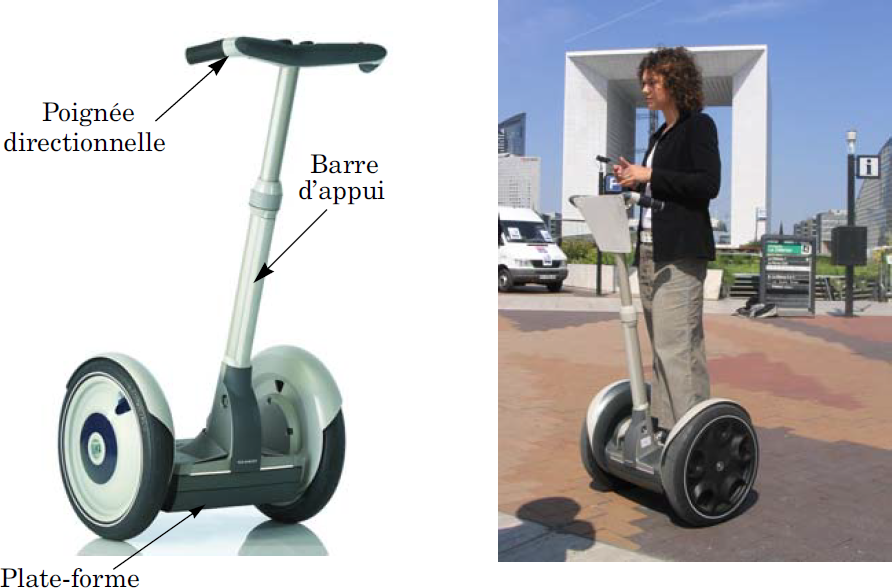
\includegraphics[width=0.7\linewidth]{ph_01}
\caption{Segway \label{ph_01}}
\end{figure}


La spécificité de ce véhicule est d’avoir deux roues qui ont le même axe de rotation, avec son centre de gravité situé au dessus de l’axe commun des roues, si bien qu’on se demande comment rester à l’équilibre une fois monté sur la plate-forme. Tout comme le cerveau permet à l’homme de tenir debout sans tomber grâce à l’oreille interne, le système comporte un dispositif d’asservissement d’inclinaison, maintenant la plate forme du véhicule à l’horizontale ou encore la barre d’appui, supposée orthogonale à cette plate forme, à la verticale.

Le Segway comporte à cet effet des capteurs et des microprocesseurs transmettant des consignes aux deux moteurs électriques équipant les deux roues.
\begin{obj}
L’objectif de cette étude est de vérifier le non-dérapage des roues en virage, les performances de vitesse et d’accélération et enfin la stabilité en ligne droite.
\end{obj}
Les exigences auxquelles doit répondre le Segway sont présentées \autoref{fig_01}.



\begin{figure}[H]
\centering
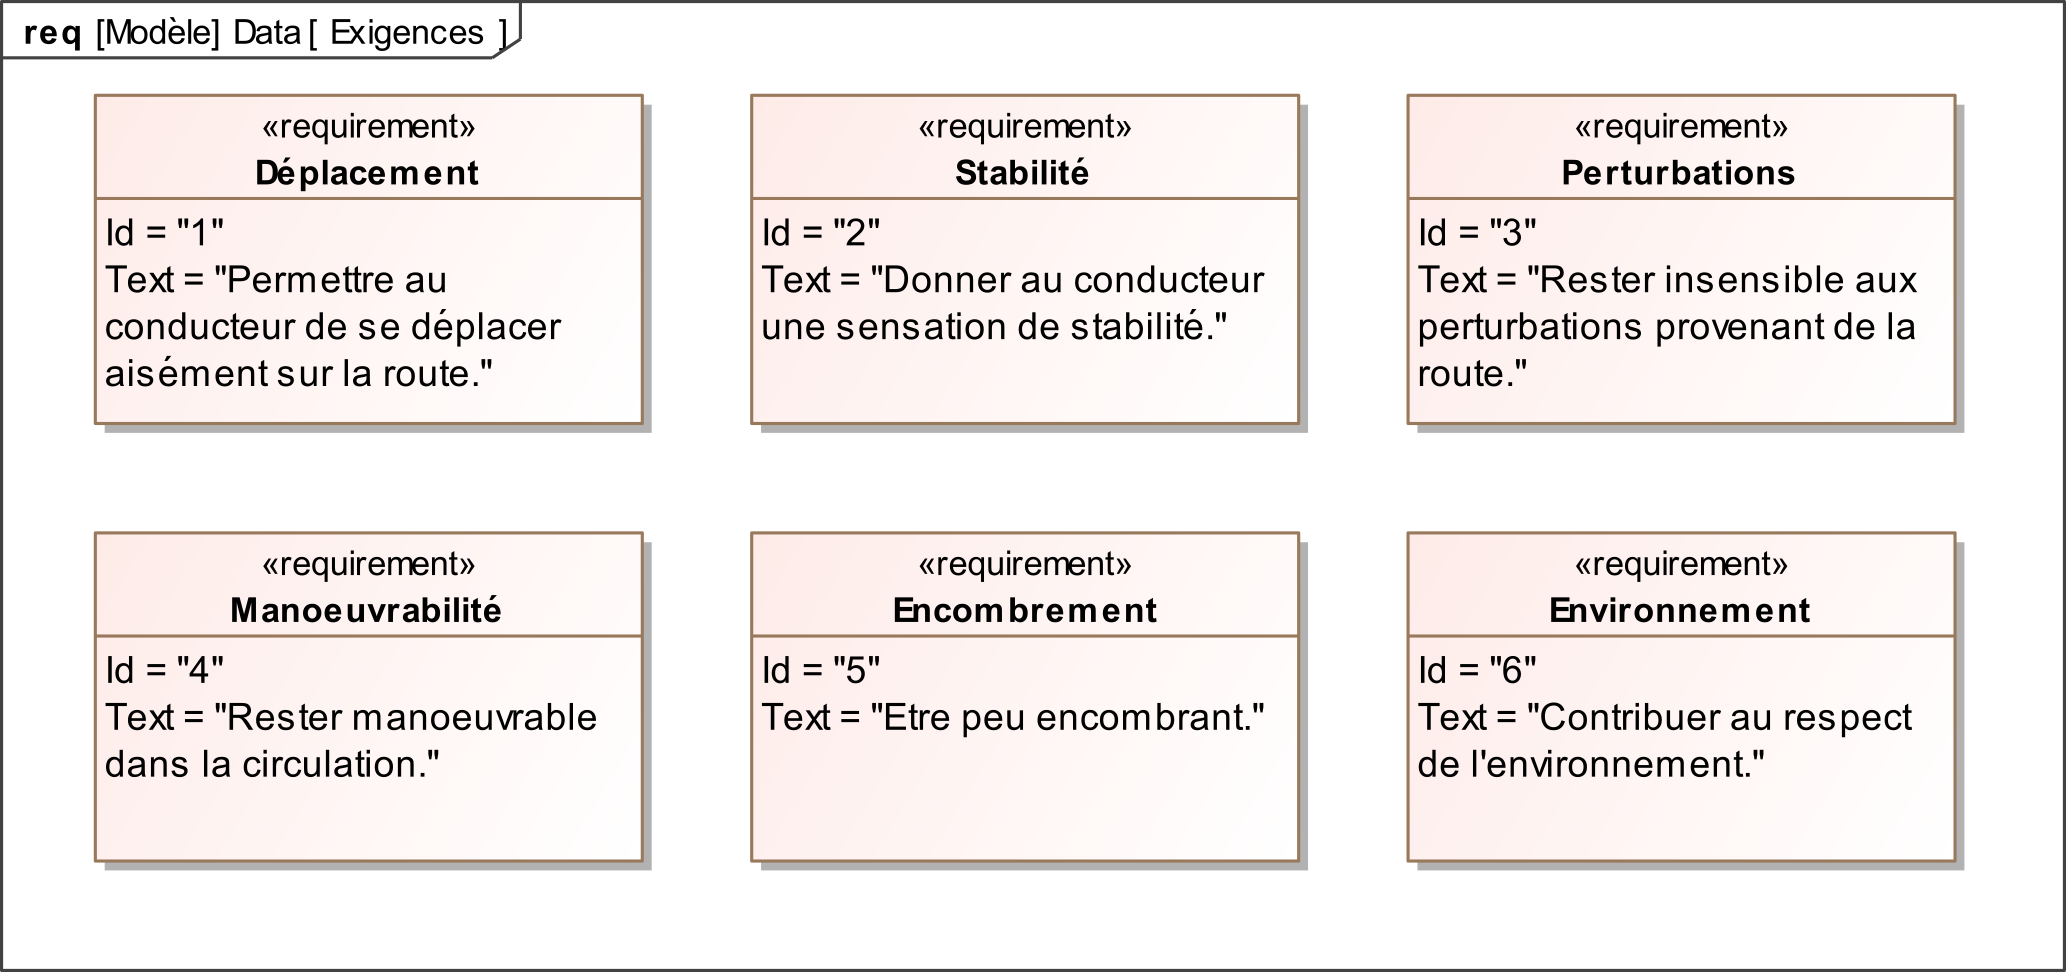
\includegraphics[width=0.9\linewidth]{req_all}
\caption{Exigences partielles \label{fig_01}}
\end{figure}

%\subsubsection*{Enoncé des fonctions de service}
%
%\begin{itemize}
%\item FS1 : Permettre au conducteur de se déplacer aisément sur la route
%\item FS2 : Donner au conducteur une sensation de stabilité
%\item FS3 : Rester insensible aux perturbations provenant de la route
%\item FS4 : Rester manœuvrable dans la circulation
%\item FS5 : Être peu encombrant
%\item FS6 : Contribuer au respect de l’environnement
%\end{itemize}

La caractérisation de chacune des exigences sera donnée au début de chaque partie.
On propose de s’appuyer sur une description structurelle du véhicule, composé (voir \autoref{fig_02}) :
\begin{itemize}
\item d’un chariot (châssis + 2 roues uniquement), transportant le conducteur;
\item de deux moto-réducteurs entraînant les roues (un par roue);
\item d’un ensemble constitué d’un gyromètre et d’un pendule délivrant une information sur l’angle d’inclinaison du châssis par rapport à la verticale et sur sa dérivée;
\item d’un calculateur élaborant, à partir des informations issues des capteurs, les consignes de commande des groupes moto-réducteurs;
\item de batteries fournissant l’énergie aux divers composants.
\end{itemize}



\begin{figure}[H]
\centering
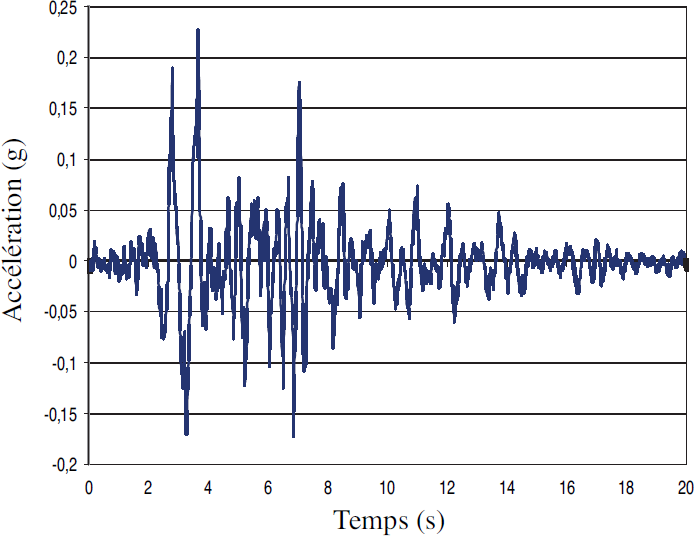
\includegraphics[width=.8\linewidth]{fig_02}
\caption{Schéma d’organisation structurelle \label{fig_02}}
\end{figure}
\fi
\subsection{Questions préliminaires}

\ifprof
\else

L’énergie maximale stockée dans les batteries vaut $E_b = \SI{2}{MJ}$. Les moto-réducteurs ont un rendement global de 0,8. La résistance moyenne à l’avancement du véhicule peut être assimilée à un effort de \SI{60}{N}.
\fi 


\question{\label{q_01}Déterminer la distance maximale que peut parcourir le Segway entre deux recharges des batteries. Justifier la pertinence de ce moyen de transport.}
\ifprof
\begin{corrige}

En tenant compte du rendement, chaque moteur délivre un travail moyen de $\eta E_b/2 = \SI{0,8}{MJ}$.

Le travail fourni par les moteurs étant égale au travail pour parcourir la distance $d$, on a $W_{d}=60d$. 
En conséquence, $d = \dfrac{\eta E_b}{60} \simeq \SI{26,6e3}{m}$ soient $\SI{26,6}{km}$.

Cette distance est compatible avec une utilisation quotidienne en milieu urbain.
\end{corrige}
\else
\fi
 
 \ifprof
 \else
Le schéma d’organisation structurelle comporte des codeurs incrémentaux, fournissant au calculateur une image de la vitesse de rotation des moteurs.
\fi

\question{\label{q_02}Rappeler en quelques lignes le principe de fonctionnement d’un codeur incrémental. Citer aussi un autre moyen d’acquisition d’une vitesse de rotation.}
\ifprof
\begin{corrige} ~\\

\begin{figure}[H]
\centering
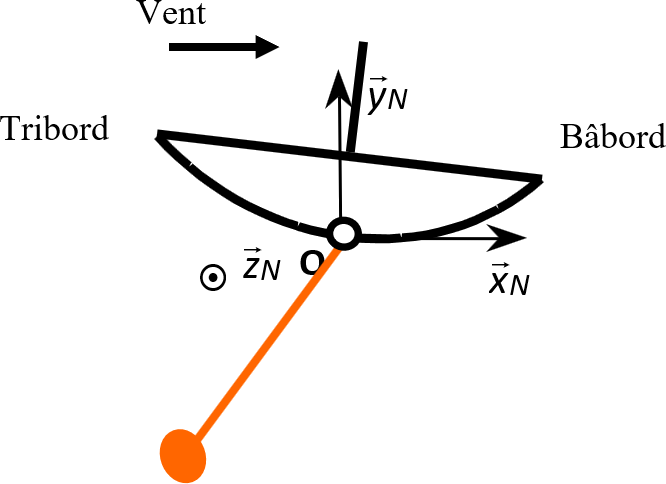
\includegraphics[width=0.7\linewidth]{cor_01}
%\caption{Segway \label{ph_01}}
\end{figure}

Un codeur absolu est composé d’un disque comportant :
\begin{itemize}
\item une piste composée de fentes espacés régulièrements sur sa périphérie ;
\item une seconde piste composée d’une seule fente permettant de faire une remise à zéro ;
\item 3 couples diode/photorésistances (ou technologie équivalente) :
\begin{itemize}
\item deux repérant les fentes sur la périphérie (décalées d’un quart de fente) ;
\item une repérant la fente de la seconde piste.
\end{itemize}
\end{itemize}
En détectant les fentes sur la piste extérieure, il est possible de détecter la position angulaire et le sens de rotation. 
La piste intérieure permet d’identifier une référence.

On peut noter que pour le sens 1 : 
$S_1 = \uparrow L_1 \cdot \overline{L_2} + \downarrow L_1 \cdot {L_2} +  \uparrow L_2 \cdot {L_1} + \downarrow L_2 \cdot \overline{L_1}$ et pour le sens 2
$S_2 = \downarrow L_1 \cdot \overline{L_2} + \uparrow L_1 \cdot {L_2} +  \downarrow L_2 \cdot {L_1} + \uparrow L_2 \cdot \overline{L_1}$.

Ainsi pour un codeur de $n$ fentes avec 2 led en quadrature, la résolution sera de $\dfrac{360}{4n}$.

En comptant le nombre de tops et connaisasnt le temps, on peut en déduire la vitesse. 

Pour mesurer une vitesse de rotation, on peut aussi utiliser une génératrice tachymétrique. 

\end{corrige}
\else
\fi

\question{\label{q_03}Rappeler quelle est la grandeur physique mesurée par un gyromètre mécanique et le principe de la mesure associé.}
\ifprof
\begin{corrige}

Un gyromètre permet de mesurer une vitesse de rotation. Principe de la mesure ?
\end{corrige}
\else
\fi
%
%Le système étudié est l’ensemble mobile (chariot, moto-réducteurs, capteurs, calculateur et batteries), sans le conducteur. Son diagramme SADT A-0 est donné figure \autoref{fig_03}.
%
%\begin{figure}[H]
%\centering
%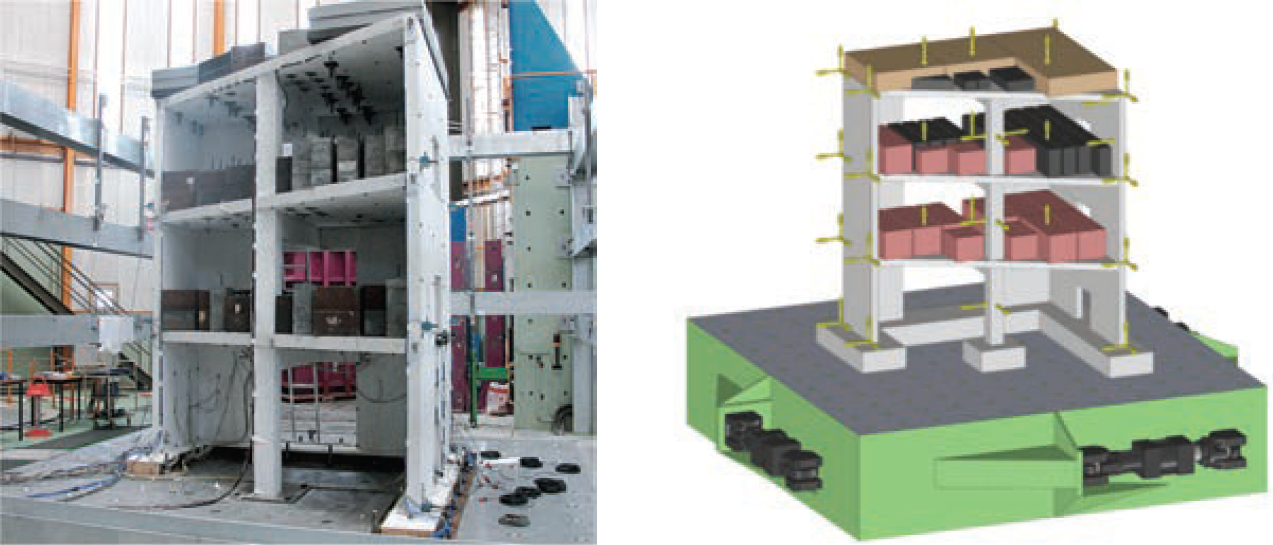
\includegraphics[width=0.7\linewidth]{fig_03}
%\caption{Diagramme A-0 du Segway \label{fig_03}}
%\end{figure}


\question{\label{q_04}Compléter la chaîne fonctionnelle associée au Segway (voir document réponse).}
\ifprof
\begin{corrige} ~\\
\begin{figure}[H] 
\centering
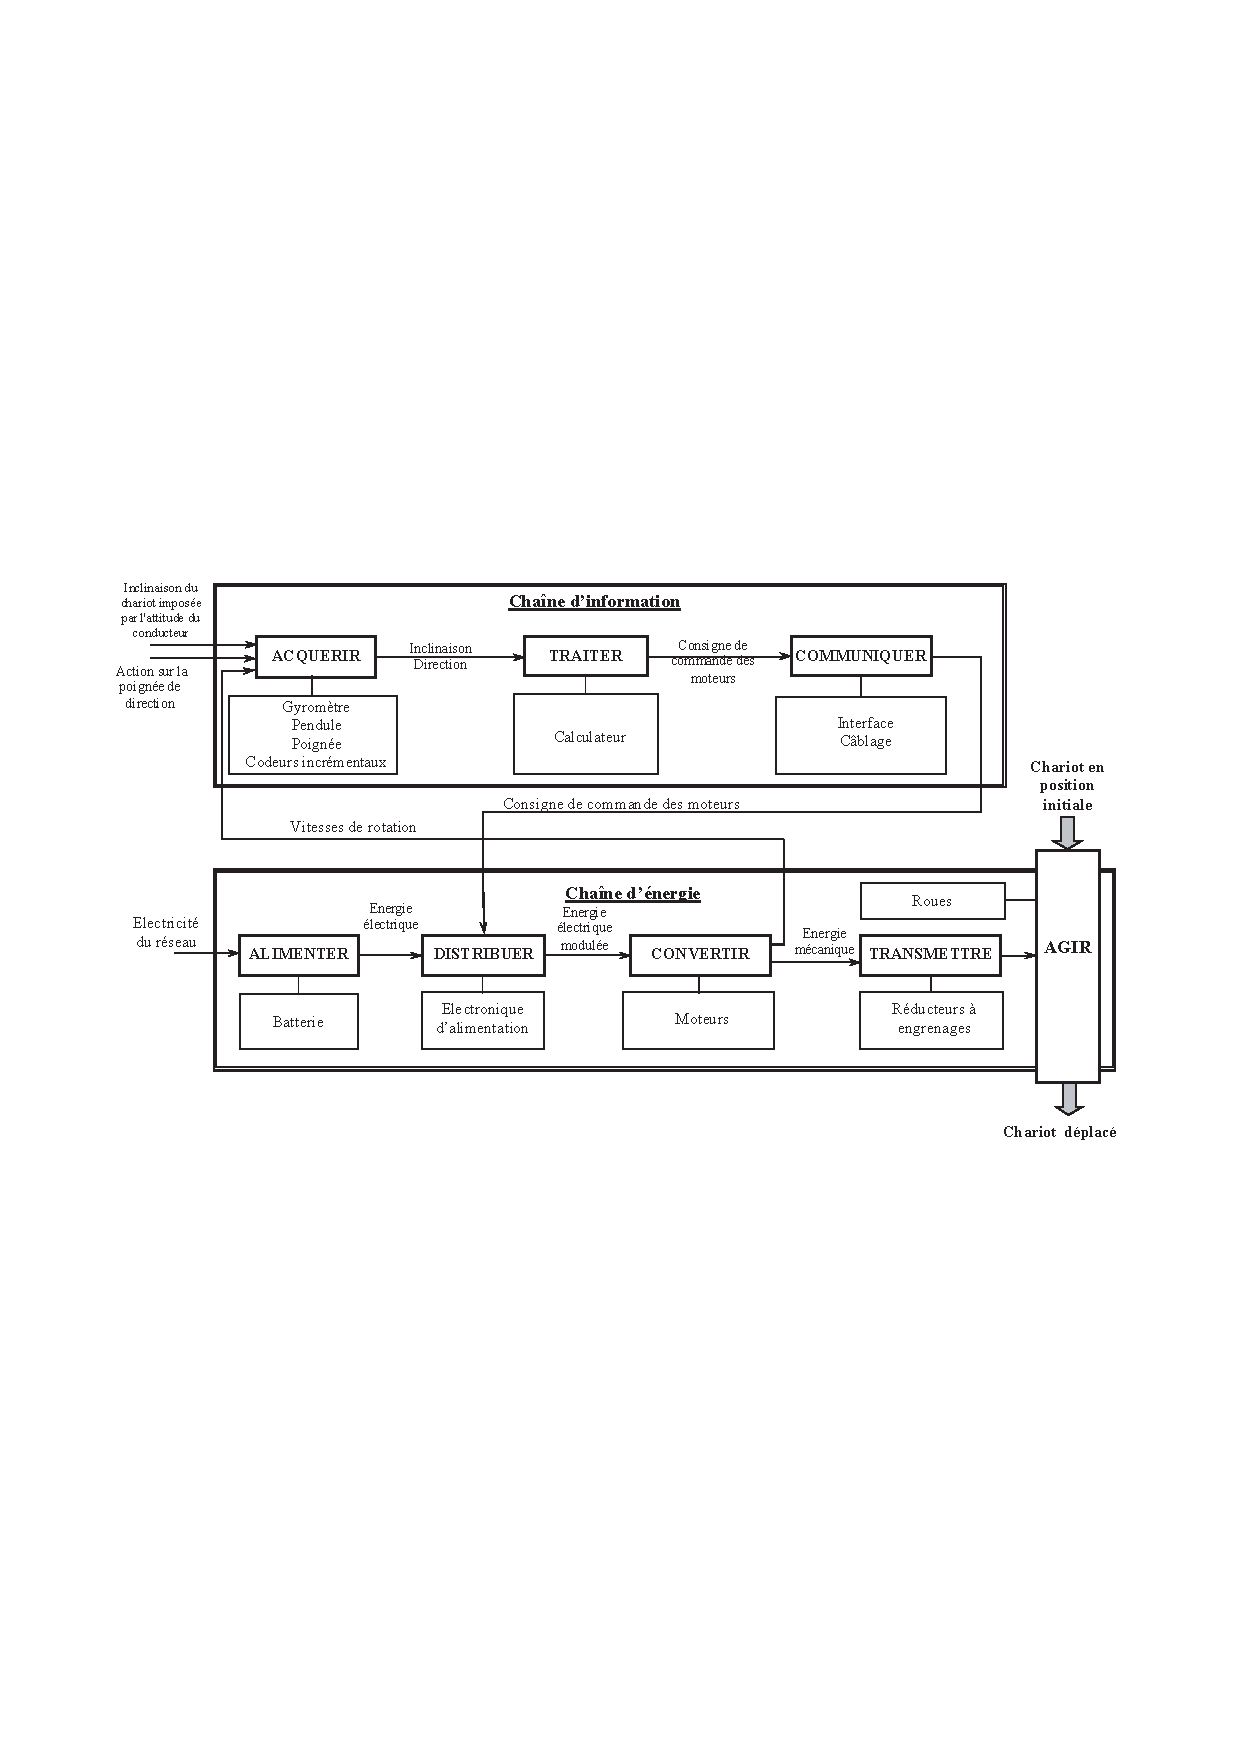
\includegraphics[width=\linewidth]{dr_01_corr}
\end{figure}
\end{corrige}
\else
\fi


\section{Modèle de comportement mécanique}
\begin{obj}
Proposer des relations cinématiques entre les paramètres du mouvement.
\end{obj}

\subsection{Modèle et paramétrage}

\ifprof
\else

\begin{itemize}
\item Soit $\mathcal{R}_0\left(O,\vect{x_0},\vect{y_0},\vect{z_0} \right)$  un repère supposé galiléen lié à la route tel que $\vect{z_0}$ soit dirigé suivant la verticale ascendante.
\item Soit $\mathcal{R}_1\left(A,\vect{x_1},\vect{y_1},\vect{z_0} \right)$ un repère en rotation par rapport à $\mathcal{R}_0$  autour de $\vect{z_0}$  tel que $\vect{x_1}$ soit colinéaire à l’axe commun des roues et $A$ le point milieu de l’axe des roues. On pose $\phi=\left(\vect{x_0},\vect{x_1}\right)=\left(\vect{y_0},\vect{y_1}\right)$  l’angle de virage.
\item Soit $\mathcal{R}_2\left(A,\vect{x_1},\vect{y_2},\vect{z_2} \right)$ un repère lié au châssis du chariot, en rotation autour de $\left(A,\vect{x_1}\right)$ par rapport à  $\mathcal{R}_1$  tel que $\vect{z_2}$  soit colinéaire à la barre d’appui. On pose  $\psi=\left(\vect{y_1},\vect{y_2}\right)=\left(\vect{z_0},\vect{z_2}\right)$  l’angle d’inclinaison du châssis par rapport à la verticale. L’asservissement consiste à maintenir cet angle nul.
\item Soit $\mathcal{R}_3\left(A,\vect{x_1},\vect{y_3},\vect{z_3} \right)$ un repère intermédiaire en rotation par rapport à $\mathcal{R}_2$, autour de  $\left(A,\vect{x_1}\right)$. On pose $\alpha=\left(\vect{y_2},\vect{y_3}\right)=\left(\vect{z_2},\vect{z_3}\right)$ l’angle d’inclinaison arrière-avant du conducteur.
\item Soit $\mathcal{R}_4\left(A,\vect{x_4},\vect{y_3},\vect{z_4} \right)$ un repère lié au conducteur, considéré comme un solide indéformable, en rotation par rapport à $\mathcal{R}_3$ autour de $\left(A,\vect{y_3}\right)$ tel que l’axe $\left(A,\vect{z_4}\right)$ passe par le centre de gravité $G$ du conducteur. On pose $\beta=\left(\vect{x_3},\vect{x_4}\right)=\left(\vect{z_3},\vect{z_4}\right)$ l’angle d’inclinaison gauche-droite du conducteur et $\vect{AG}=h\vect{z_4}$ avec $h$ constante positive.
\item Soit $\mathcal{R}_D\left(O_D,\vect{x_1},\vect{y_D},\vect{z_D} \right)$ un repère lié à la roue Droite, en rotation autour de $\left(A,\vect{x_1}\right)$  par rapport à $\mathcal{R}_2$ où $O_D$ est le centre de gravité de la roue droite.  
$\theta_D=\left(\vect{y_2},\vect{y_D}\right)=\left(\vect{z_2},\vect{z_D}\right)$ est l’angle de rotation de la roue droite par rapport au châssis. $I_D$ est le point de contact de la roue droite avec la route tel que  $\vect{I_D O_D}=R\vect{z_0}$. On suppose que la roue droite roule sans glisser sur le sol au point  $I_D$.
\item Soit $\mathcal{R}_G\left(O_G,\vect{x_1},\vect{y_G},\vect{z_G} \right)$ un repère lié à la roue Gauche, en rotation autour de $\left(A,\vect{x_1}\right)$  par rapport à $\mathcal{R}_2$ où $O_G$ est le centre de gravité de la roue gauche.  
$\theta_G=\left(\vect{y_2},\vect{y_G}\right)=\left(\vect{z_2},\vect{z_G}\right)$ est l’angle de rotation de la roue gauche par rapport au châssis. $I_G$ est le point de contact de la roue gauche avec la route et on suppose que la roue gauche roule sans glisser sur le sol au point $I_G$ (les deux roues ont même rayon $R$).
\end{itemize}

On note $L$ l’empattement du chariot tel que $\vect{O_DO_G}=L\vect{x_1}$ et $\vect{O_D A}=\dfrac{L}{2}\vect{x_1}=\vect{AO_G}$.


Un paramétrage simplifié est donné fans la partie droite de la \autoref{fig_04} ($\beta=0$ c'est-à-dire $\vect{z_3}=\vect{z_4}$).
\begin{figure}[H]
\centering
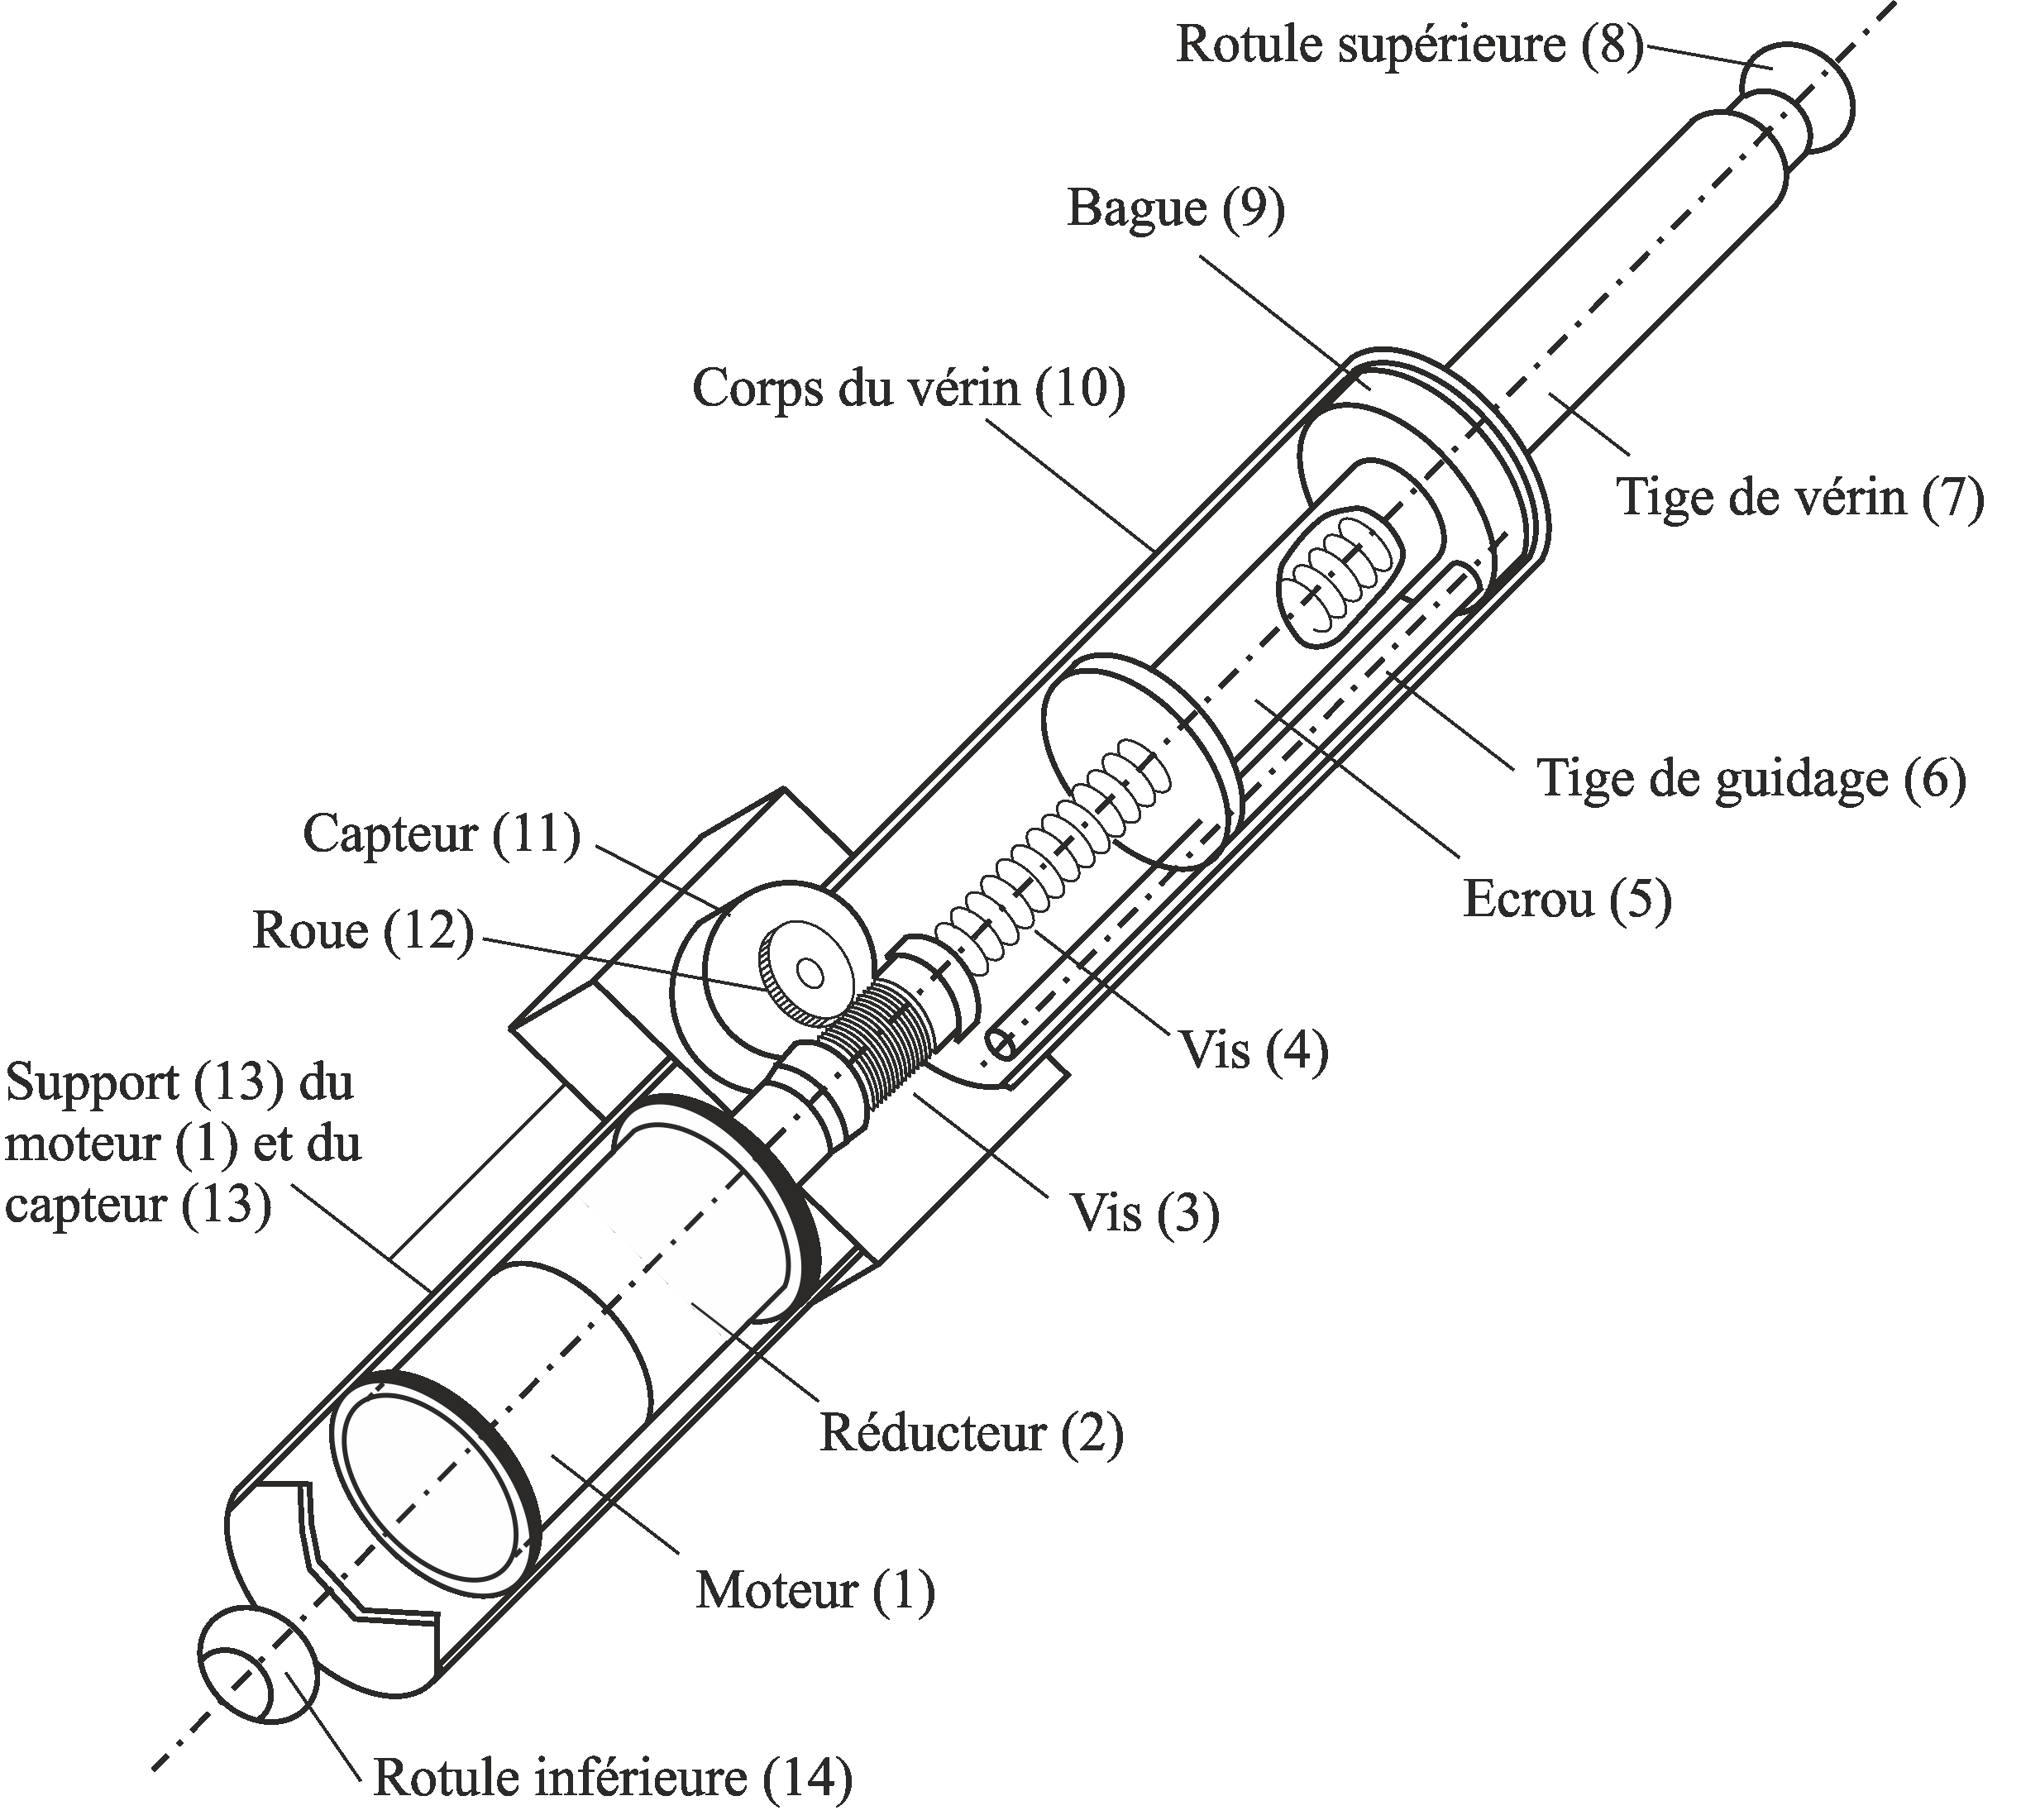
\includegraphics[width=0.9\linewidth]{fig_04}
\caption{Paramétrage cinématique du système \label{fig_04}}
\end{figure}
\fi


\subsection{Etude cinématique préalable}
\question{\label{q_05}Proposer un graphe des liaisons du système restreint à l’ensemble de solides \{Route, Roue Gauche, Roue Droite, Châssis\}. Préciser pour chaque liaison ses caractéristiques géométriques.}
\ifprof
\begin{corrige}~\\
\begin{figure}[H]
\centering
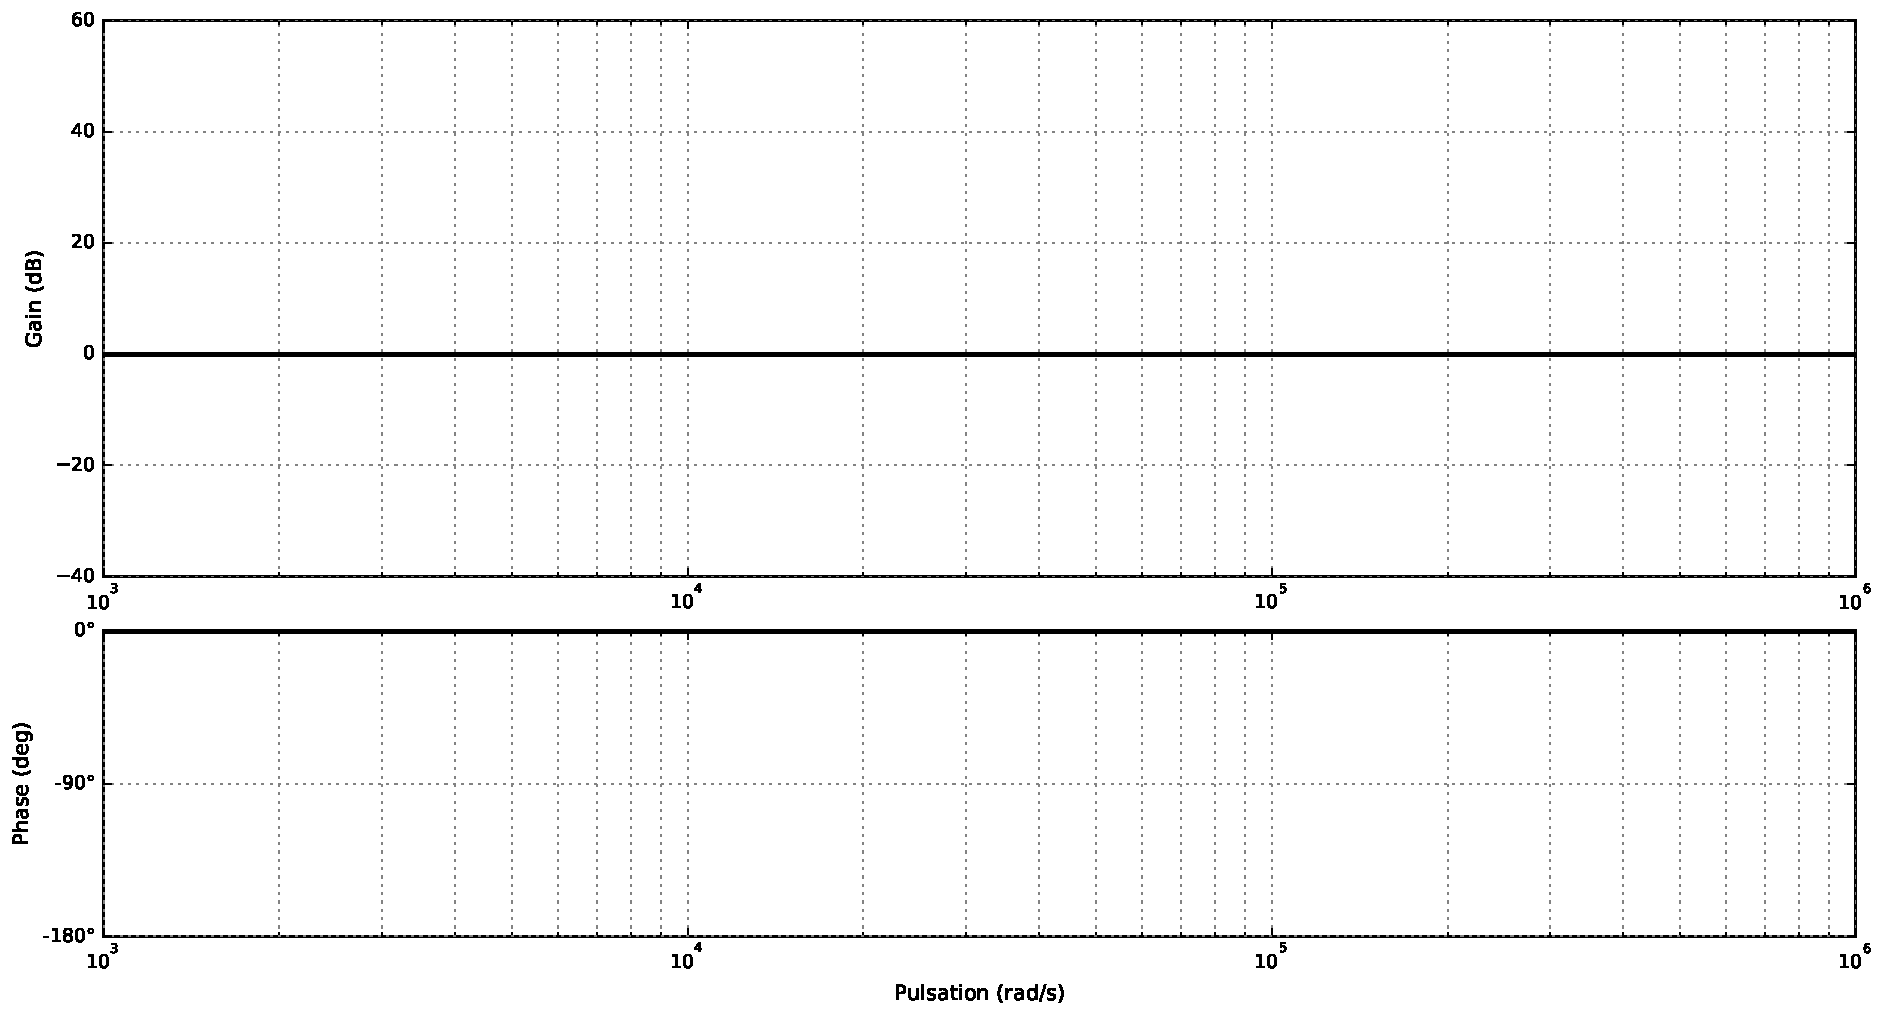
\includegraphics[width=0.45\linewidth]{cor_02}
%\caption{Segway \label{ph_01}}
\end{figure}
\end{corrige}
\else
\fi

\question{\label{q_06}En s’appuyant sur le paramétrage et en utilisant de la couleur, proposer un schéma cinématique du système \{Roue Gauche, Roue Droite, Plate forme, Conducteur\}, en complétant l’épure du document réponse (ne pas schématiser le contact roue/route).}
\ifprof
\begin{corrige} ~\\
\begin{figure}[H]
\centering
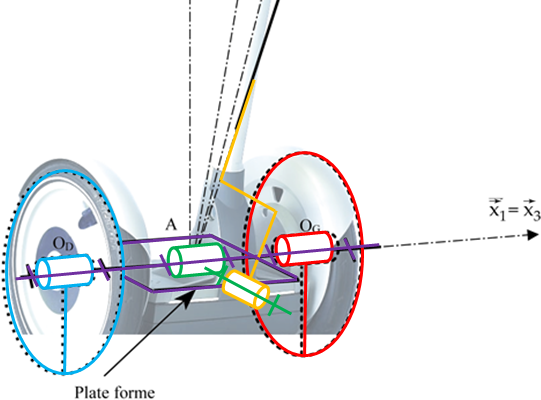
\includegraphics[width=0.6\linewidth]{cor_03}
%\caption{Segway \label{ph_01}}
\end{figure}
\end{corrige}
\else
\fi

\question{\label{q_07}Exprimer, en fonction du paramétrage, les torseurs cinématiques :}
\textit{
\begin{itemize}
\item du châssis par rapport au sol : $\torseurcin{V}{2}{0}$, en notant $\vectv{A}{2}{0} = U\vect{x_1}+V\vect{y_1}$;
\item de la roue droite par rapport au châssis : $\torseurcin{V}{R_D}{2}$;
\item de la roue droite par rapport au châssis : $\torseurcin{V}{R_G}{2}$.
\end{itemize}}
\ifprof
\begin{corrige}
On a $\torseurcin{V}{2}{0} = \torseurl{\vecto{2}{0}}{\vectv{A}{2}{0}}{A}$ avec 
$\vectv{A}{2}{0} = U\vect{x_1}+V\vect{y_1}$ et 
$\vecto{2}{0} = \vecto{2}{1}+\vecto{1}{0} = \dot{\psi}\vect{x_{12}}+\dot{\phi}\vect{z_{01}}$.
On a donc  $\torseurcin{V}{2}{0} = \torseurl{\dot{\psi}\vect{x_{12}}+\dot{\phi}\vect{z_{01}}}{U\vect{x_1}+V\vect{y_1}}{A}$.

De plus  $\torseurcin{V}{R_D}{2} = \torseurl{\dot{\theta_D}\vect{x_1}}{\vect{0}}{A}$ 
et $\torseurcin{V}{R_G}{2} = \torseurl{\dot{\theta_G}\vect{x_1}}{\vect{0}}{A}$ .

\end{corrige}
\else
\fi


\question{\label{q_08}\'Enoncer ensuite les deux relations de roulement sans glissement des roues par rapport à la route et déterminer trois relations scalaires liant les 6 paramètres inconnus $\dot{\psi}$, $\dot{\phi}$, $\dot{\theta}_R$, $\dot{\theta}_G$ $U$ et $V$ aux dimensions $L$ et $R$.}
\ifprof
\begin{corrige}
En exploitant le roulement sans glissement au point $I_D$, on a $\vectv{I_D}{R_D}{0}=\vect{0}$. 
On a alors $\vectv{A}{R_D}{0} = \vectv{I_D}{R_D}{0} + \vect{A I_D} \wedge \vecto{R_D}{0}$.

Or, $\vecto{R_D}{0}= \vecto{R_D}{2}+\vecto{2}{0}$ $=\dot{\theta_D}\vect{x_1}+\dot{\psi}\vect{x_{12}}+\dot{\phi}\vect{z_{01}}$.

On a donc 
$\vectv{A}{R_D}{0} = \left(-\dfrac{L}{2}\vect{x_1}-R\vect{z_1}\right)\wedge \left(\dot{\theta_D}\vect{x_1}+\dot{\psi}\vect{x_{12}}+\dot{\phi}\vect{z_{01}}\right)$

$=\left(-\dfrac{L}{2}\vect{x_1}\right)\wedge \left(\dot{\theta_D}\vect{x_1}+\dot{\psi}\vect{x_{12}}+\dot{\phi}\vect{z_{01}}\right)+\left(-R\vect{z_1}\right)\wedge \left(\dot{\theta_D}\vect{x_1}+\dot{\psi}\vect{x_{12}}+\dot{\phi}\vect{z_{01}}\right)$

$=\left(-\dfrac{L}{2}\vect{x_1}\right)\wedge \left(\dot{\phi}\vect{z_{01}}\right)+\left(-R\vect{z_1}\right)\wedge \left(\dot{\theta_D}\vect{x_1}+\dot{\psi}\vect{x_{12}}\right)$
$=\dfrac{L}{2}\dot{\phi}\vect{y_{1}}-R\left(\dot{\theta_D}+\dot{\psi}\right)\vect{y_1}$

De même, $\vectv{A}{R_G}{0}=-\dfrac{L}{2}\dot{\phi}\vect{y_{1}}-R\left(\dot{\theta_G}+\dot{\psi}\right)\vect{y_1}$.


Or, $\vectv{A}{2}{0} = \vectv{A}{2}{R_D} + \vectv{A}{R_D}{0}$ et $\vectv{A}{2}{R_D} = \vect{0}$ (axe de la liaison pivot; donc $\vectv{A}{2}{0} = \vectv{A}{R_D}{0} = \vectv{A}{R_G}{0}$ et 
$
\left\{
\begin{array}{l}
V = \dfrac{L}{2}\dot{\phi}-R\left(\dot{\theta_D}+\dot{\psi}\right) \\
V = -\dfrac{L}{2}\dot{\phi}-R\left(\dot{\theta_G}+\dot{\psi}\right) \\
U = 0
\end{array}
\right.
$.
\end{corrige}
\else
\fi

\subsection{\'Etude de la transmission de puissance}
\ifprof
\else

La transmission de puissance choisie possède deux moteurs électriques (un pour chaque roue), associé chacun à un réducteur de rapport de réduction  $|K_R| =\dfrac{1}{24}$.
\fi

\question{\label{q_09}Une voiture ne possède généralement qu’un seul moteur et qu’un seul réducteur (la boîte de vitesses). Le différentiel permet de répartir la puissance motrice sur les deux roues motrices. Expliquez pourquoi le constructeur du Segway n’a pas adopté cette solution.}
\ifprof
\begin{corrige}
Les organes mécaniques (réducteur, différentiel) présentent un coût supérieur à celui du coût d'un moteur et d'un variateur de vitesse. Il faudra cependant s'assurer que la commande soit suffisamment précise pour ne pas créer de déviation dans les trajectoires (une vitesse différente pour chacune des roues en ligne droite conduirait à des écarts de trajectoire).
\end{corrige}
\else
\fi

\ifprof
\else

Un pré-dimensionnement des réducteurs a conduit à adopter les contraintes suivantes :
\begin{itemize}
\item $[OO_M]=\SI{90}{mm}$ (voir document réponse);
\item module $m=\SI{1}{mm}$  pour tous les engrenages;
\item nombre de dents minimum pour chaque roue dentée : $Z_{i \text{mini}}=15$. 
\end{itemize}

Les points $O$ et $O_M$ correspondent respectivement aux projections, dans le plan $\left( O_D,\vect{y_2},\vect{z_2}\right)$ , des axes de rotation d’une roue et du moteur associé.
\fi

\question{\label{q_10}Proposer, sur le document réponse, une architecture du réducteur s’intégrant dans le carter et dont le rapport de réduction vaut $|K_R| =\dfrac{1}{24}$ en dessinant une épure de la solution adoptée. Représenter uniquement les diamètres primitifs des roues dentées, dans le plan du document réponse puis récapituler sous forme de tableau, sur votre copie, les nombres de dents choisis.}
\ifprof
\begin{corrige}
Le nombre de dents minmal est de 15 dents soit un diamètre primitif de \SI{15}{mm}.
Pour avoir un rapport de 24, un pignon moteur doit entrainer un pignon récepteur de \SI{360}{mm}. Dans ce cas, l'entraxe serait alors de $\dfrac{360}{2}+\dfrac{15}{2} > \SI{90}{mm}$.

Une des solutions consisterait donc à utiliser un train d'engrenages. Essayons de mettre en équation le problème : 
\begin{itemize}
\item dans ce cas, il y a 4 inconnues, à savoir les diamètres primitifs (ou nombre de dents car $d=mZ$) des 4 roues dentées;
\item la condition d'entraxe se traduit par $\dfrac{D_1}{2} + \dfrac{D_{22}}{2}+ \dfrac{D_{21}}{2}+ \dfrac{D_{3}}{2} = \ell = \SI{90}{mm}$;
\item le rapport de réduction se traduit par $\dfrac{D_1 D_{21}}{D_3 D_{22}} = \dfrac{1}{K_R}= \dfrac{1}{24}$.
\end{itemize}
Dans ces conditions on a 2 équations pour 4 inconnues. Fixons deux inconnues : $D_1 =  D_{21} = \SI{15}{mm}$. 
On a alors $\dfrac{D_1 D_{21} K_R}{D_3 } = D_{22}$ et 
 $\dfrac{D_1}{2} + \dfrac{D_1 D_{21} K_R}{2D_3 }+ \dfrac{D_{21}}{2}+ \dfrac{D_{3}}{2} = \ell$

$ \Leftrightarrow  \dfrac{D_1}{2} + \dfrac{D_1 D_{21} K_R}{2D_3 }+ \dfrac{D_{21}}{2}+ \dfrac{D_{3}}{2} = \ell$

$ \Leftrightarrow  D_1 D_3  + D_1 D_{21} K_R+D_{21}D_3 + D_{3}^2 = 2 D_3\ell$.

On a donc $D_{3}^2 + D_3\left(- 2\ell + D_1+ D_{21} \right) + D_1 D_{21} K_R= 0$.

On a alors  $ \Delta  = \left(- 2\ell + D_1+ D_{21} \right)^2 - 4  D_1 D_{21} K_R$. 

AN : $\Delta = \left(- 2\times 90+ 15 + 15  \right)^2 - 4  \times 15\times 15 \times {24} = 30^2 $.

On a donc $D_3 = \dfrac{-\left(- 2\ell + D_1+ D_{21} \right)\pm\sqrt{\Delta}}{2}$.
Soit $D_3 = \SI{90}{mm}$ ou $D_3 = \SI{60}{mm}$.

Par suite,  $D_{22}=\dfrac{D_1 D_{21} K_R}{D_3 }$; donc 
 si $D_3 = \SI{90}{mm}$ alors $D_{22}=\SI{60}{mm} $
et  si $D_3 = \SI{60}{mm}$ alors $D_{22}= \SI{90}{mm}$.


\begin{figure}[H]
\centering
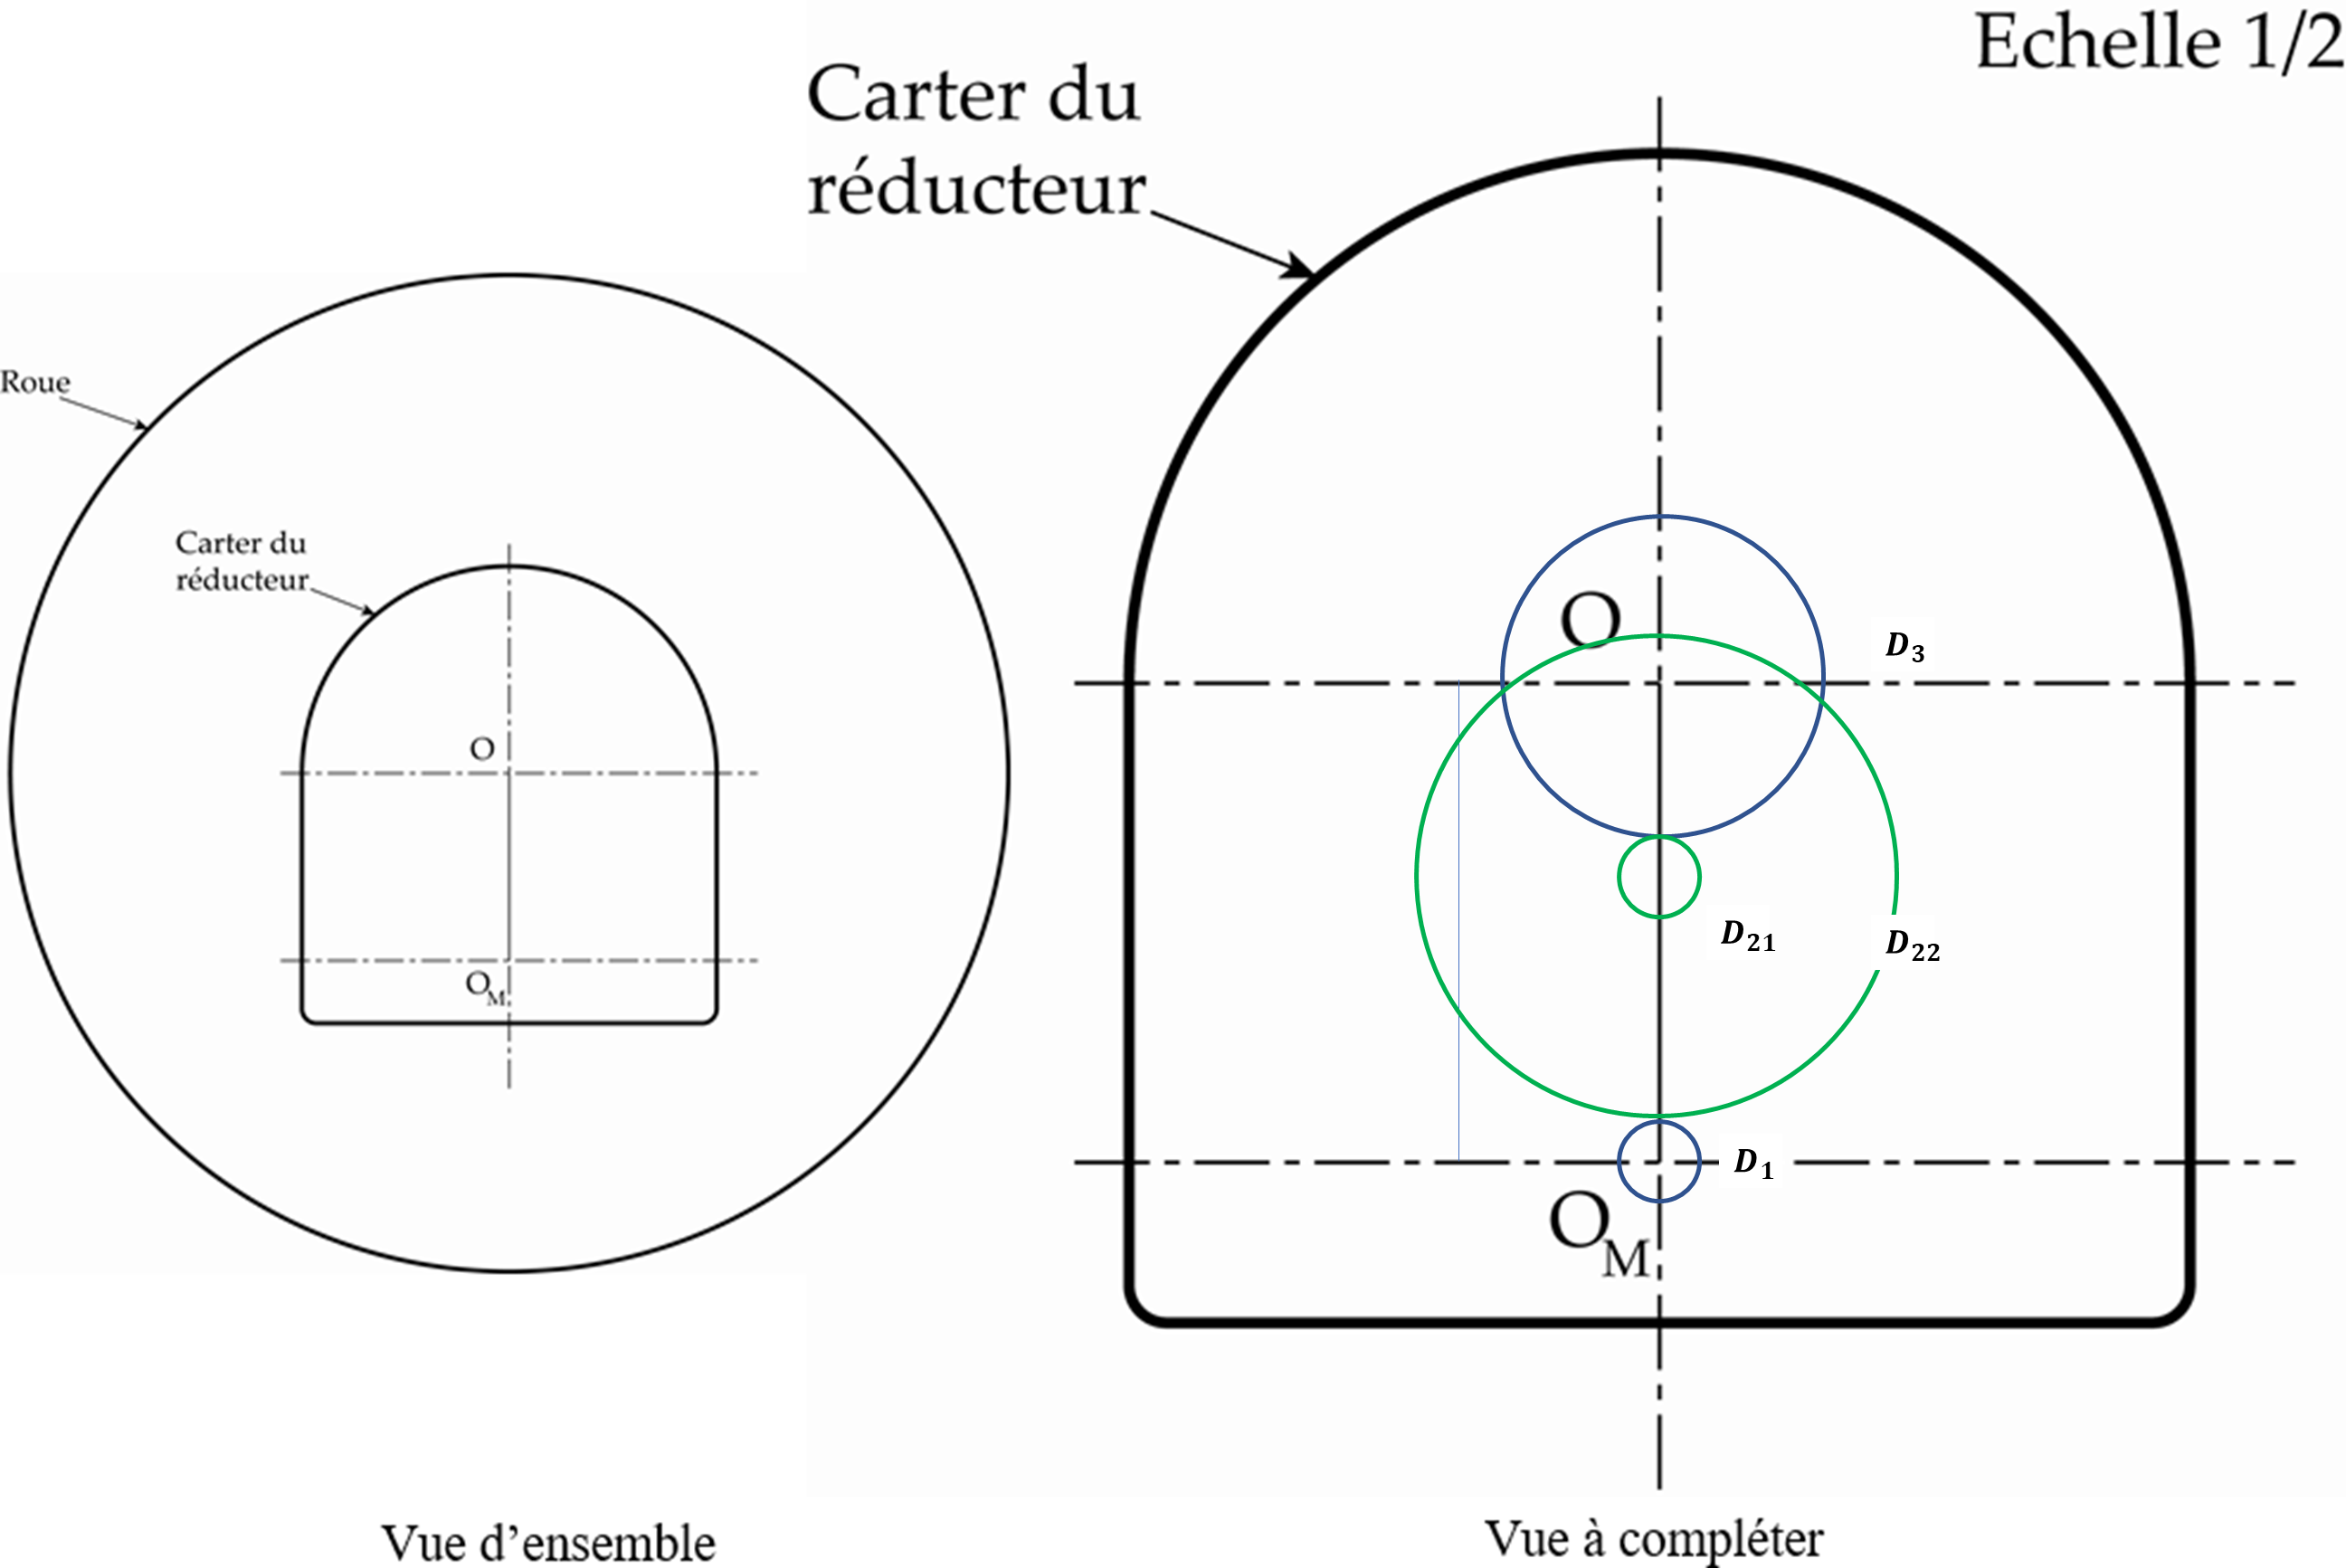
\includegraphics[width=0.9\linewidth]{cor_07}
\end{figure}


\end{corrige}
\else
\fi



\section{Validation de l'exigence 4 : rester man\oe{}uvrable dans la circulation}
\begin{obj}
Vérifier le non dérapage des roues et le non basculement du Segway pour les différents rayons de virage.
\end{obj}
\ifprof
\else

Le dérapage se définit comme le glissement suivant $\vect{x_1}$ ou $\vect{y_1}$ des roues par rapport à la route et le basculement du Segway a lieu lorsque l’une des roues n’est plus en contact avec la route. Trois configurations de vitesse du Segway sont étudiées :
\begin{itemize}
\item déplacement à la vitesse d’un homme marchant;
\item déplacement à la vitesse d’un homme courant;
\item déplacement à la vitesse maximale.
\end{itemize}

La \autoref{req_04} ci-dessous est extrait du Cahier des Charges.


\begin{figure}[H]
\centering
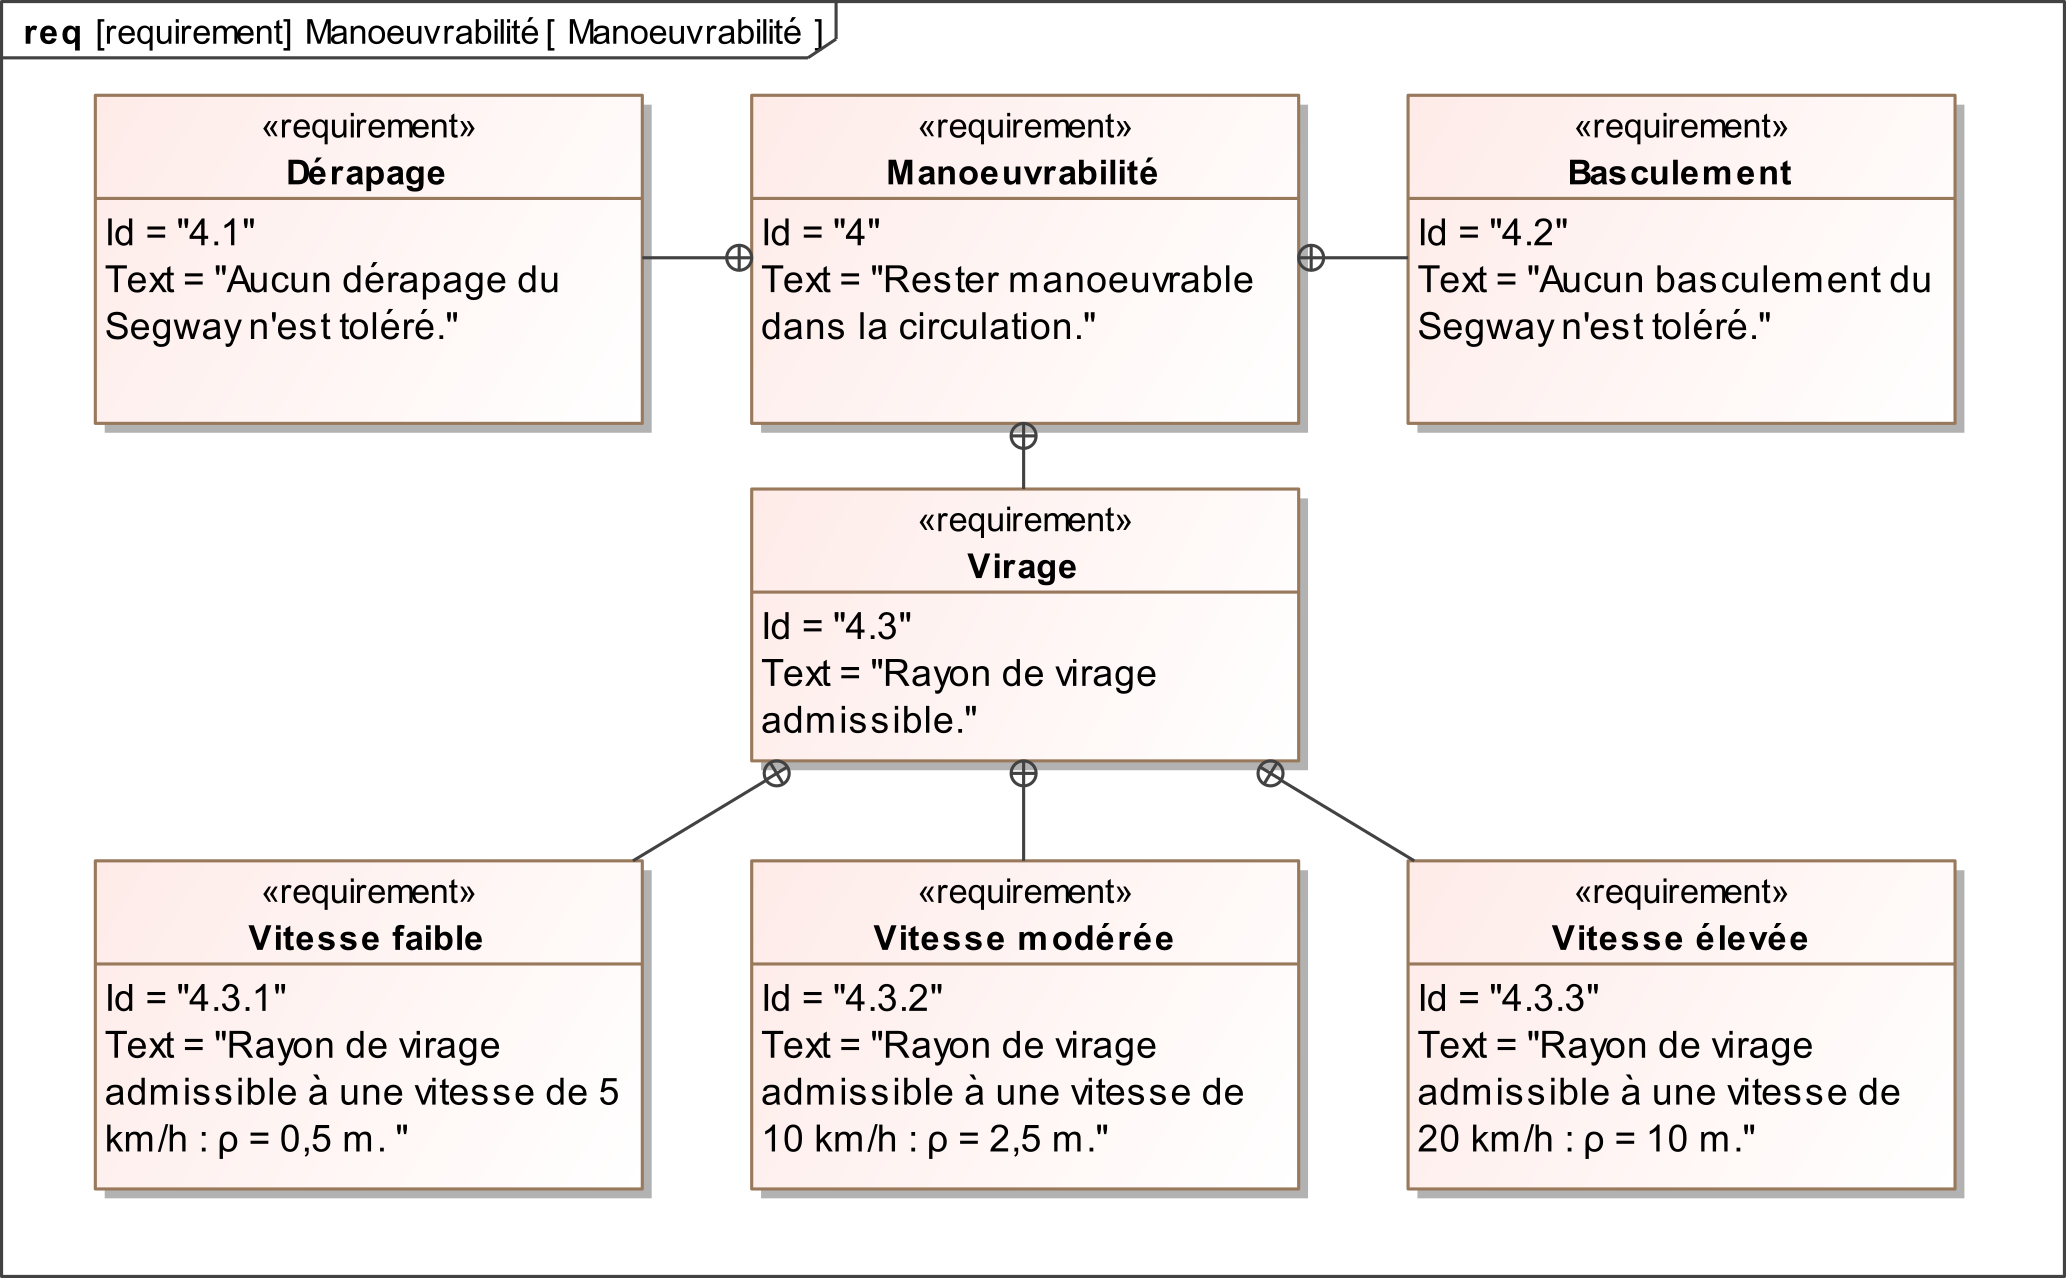
\includegraphics[width=0.9\linewidth]{req_04}
\caption{Extrait du CdCF relatif à l'exigence 4 \label{req_04} }%$\vect{z_3}=$}% $\beta = 0$ soit $\vect{z_3}=\vect{z_4}$ }
\end{figure}

\fi

\subsection{Analyse du modèle de calcul des actions mécaniques \label{sec:A}}

\ifprof
\else

Le système étudié est celui de la question \ref{q_12}, constitué des solides \{Route, Roue Gauche, Roue Droite, Châssis\}. Seuls les paramètres $V$, $\phi$, $\psi$ sont variables, les autres paramètres n’intervenant pas. Les contacts roue/route en $I_G$ et $I_D$ sont modélisés par des liaisons sphère plan avec frottement (roulement sans glissement). Cette modélisation conduit aux torseurs d’actions mécaniques exercées par la route sur les roues suivants :
$\torseurstat{T}{\text{Route}}{R_{G}} = \torseurl{X_G\vect{x_1}+Y_G\vect{y_1}+Z_G\vect{z_0}}{\vect{0}}{I_G}$
  et  
$\torseurstat{T}{\text{Route}}{R_{D}} = \torseurl{X_D\vect{x_1}+Y_D\vect{y_1}+Z_D\vect{z_0}}{\vect{0}}{I_D}$.


%\question{\label{q_11}
%En s’appuyant sur le graphe des liaisons de la question \ref{q_05}, déterminer le nombre de mobilités $m$ du système \{Route, Roue Gauche, Roue Droite, Châssis\}. En déduire alors le degré d’hyperstatisme  $h$ du mécanisme.}
%\ifprof
%\begin{corrige}
%\end{corrige}
%\else
%\fi

Dans la suite de cette partie, l’asservissement d’inclinaison est considéré comme parfaitement réalisé, c’est à dire que $\psi = 0$. De plus, le conducteur est supposé uniquement incliné d’un angle $\beta$ constant vers l’intérieur du virage. On impose de plus $\alpha=0$, ce qui impose aussi  $V=$constante où $V$ est négatif en marche avant. Enfin, le virage est pris à vitesse de rotation constante soit $\dot{\phi}$=constante et $\dot{\phi}>0$.

  \fi
  
\subsection{Détermination de l’inclinaison du conducteur en virage}

\ifprof
\else

La position naturelle de l’individu en virage (cas de la bicyclette, des rollers, ...) est de s’incliner vers l’intérieur du virage. L’application du Principe Fondamental de la Dynamique au conducteur montre alors que cette condition est équivalente à $\vect{g}-\vectg{G}{4}{0}$ colinéaire à $\vect{z_4}$.

Après calcul de $\vectg{G}{4}{0}$, la figure du document réponse donne deux projections de $\vect{g}-\vectg{G}{4}{0}$ dans la base $\left(\vect{x_4},\vect{y_4},\vect{z_4} \right)$ en fonction de l’inclinaison $\beta$ du conducteur, avec les paramètres : 
$\dot{\phi}=\SI{0,8}{rad.s^{-1}}$, 
$h=\SI{0,95}{m}$, 
$g=\SI{9,81}{m.s^{-2}}$ et 
$V=-\SI{10}{km.h^{-1}}$ (soit $\rho = \SI{3,5}{m}$).

\fi

\question{\label{q_12}Par un tracé sur le document réponse, justifié sur la copie, donner alors la valeur de ${\beta}$ qui permet de vérifier la condition exposée ci-dessus.}
\ifprof
\begin{corrige}
$\vect{g}-\vectg{G}{4}{0}$ colinéaire à $\vect{z_4}$ donc la projection sur $\vect{x_4}$ doit être nulle.
Deux angles $\beta$ correspondent à cette condition : $\beta\simeq 10\degres$, $\beta\simeq -160\degres$. La configuration du système impose $\beta\simeq 10\degres$.



\begin{figure}[H]
\centering
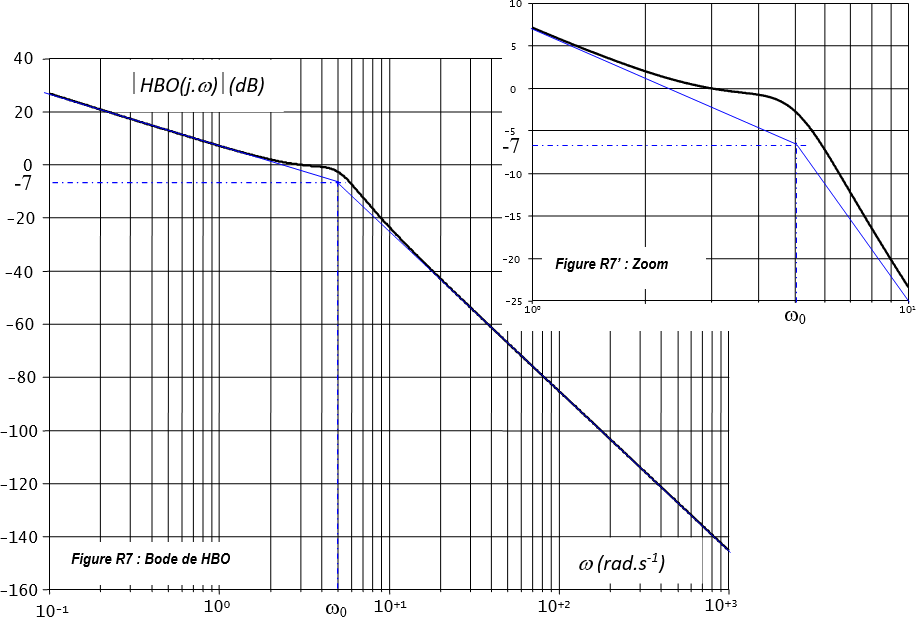
\includegraphics[width=0.6\linewidth]{cor_04}
%\caption{Extrait du CdCF relatif à l'exigence 4 \label{req_04} }%$\vect{z_3}=$}% $\beta = 0$ soit $\vect{z_3}=\vect{z_4}$ }
\end{figure}
\end{corrige}
\else
\fi


\subsection{\'Etude dynamique simplifiée du Segway en virage \label{iii:b}}

\ifprof
\else

Dans ce paragraphe, un modèle simplifié où le conducteur est assimilé à une masse concentrée $m_H$ en $G$  et le chariot  assimilé à une masse concentrée $m_s$ en $A$ est adopté. De plus, l’inertie des roues et l'inertie en rotation du Segway sont négligées devant les termes liés à la masse du conducteur et du chariot. Les hypothèses $V =$constante, $\beta =$constante, $\dot{\phi} =$constante et $\psi=0$ avec $\beta$ tel que $\vect{g}-\vectg{G}{4}{0}$ soit colinéaire à 
$\vect{z_4}$ (comme défini en \ref{iii:b}) sont conservées. On isole alors le système complet \{Conducteur, Châssis, Roue Droite, Roue Gauche\}. 
\fi

\question{\label{q_13}Faire le Bilan des Actions Mécaniques Extérieures qui s’exercent sur ce système.
}
\ifprof
\begin{corrige}
On a $\torseurstat{T}{0}{R_G}$, $\torseurstat{T}{0}{R_D}$, $\torseurstat{T}{\text{Pesanteur}}{\text{Châssis}}$ et $\torseurstat{T}{\text{Pesanteur}}{\text{Conducteur}}$.

\end{corrige}
\else
\fi

\ifprof
\else

L’application du Principe Fondamental de la Dynamique à ce système dans son mouvement par rapport au sol permet d’obtenir, après réduction au point $A$, les équations suivantes projetées sur la base $\left(\vect{x_1},\vect{y_1},\vect{z_0} \right)$ :
\begin{itemize} 
\item théorème de la résultante dynamique selon : $\quad \vect{x_1}$
$-m_H\dot{\phi} \left(V + h\dot{\phi} \sin\beta\right)-m_SV\dot{\phi} =X_G + X_D$;
\item théorème de la résultante dynamique selon $\vect{z_0}$  : $\quad 0=Z_G + Z_D - \left(m_H+m_S\right)g$;
\item théorème du moment dynamique en $A$ en projection selon $\vect{y_1}$  : $\quad \dfrac{L}{2}Z_G + RX_G - \dfrac{L}{2}Z_D + RX_D= 0$.
 \end{itemize}
 \fi
 
\question{\label{q_14}Expliquer pourquoi le système d’équations obtenu ne permet pas de déterminer toutes les inconnues d’effort et recenser celles qui ne peuvent pas être calculées sans hypothèse complémentaire.}% Expliquer l’origine de cette impossibilité.}
\ifprof
\begin{corrige}

\end{corrige}
\else
\fi



\ifprof
\else
Le modèle de frottement de Coulomb de coefficient $f$ est adopté pour le contact roue/sol, et, en raison du déchargement de la roue gauche, l’hypothèse $X_G = 0$ est adoptée.
\fi

\question{\label{q_15}Énoncer les lois de Coulomb en utilisant les notations de la partie \ref{sec:A} pour une roue, dans les cas d'adhérence et de glissement.}
\ifprof
\begin{corrige}~\\

\noindent\begin{minipage}[t]{.33\linewidth}
\begin{center}
\textbf{Cas 1 -- Glissement -- $\vectv{I}{2}{1}\neq \vect{0}$}
\end{center}

\begin{itemize}
\item Connaissant le sens et la direction de $\vectv{I}{2}{1}$, alors $\vect{t_{12}}$ s'oppose à $\vectv{I}{2}{1}$.
\item $|T_{12}| = f |N_{12}|$.
\item La vecteur vitesse appartenant au plan tangent au contact, on dit que l'effort résultant ($\vect{F_{12}}=N_{12} \vect{n_{12}}+T_{12} \vect{t_{12}}$) est sur le cône de frottement. 
\end{itemize}
\end{minipage}\hfill
\begin{minipage}[t]{.35\linewidth}
\begin{center}
\textbf{Cas 2 -- Adhérence -- $\vectv{I}{2}{1} = \vect{0}$}
\end{center}

\begin{itemize}
\item La direction de $\vect{t_{12}}$ n'est pas connue. 
\item $|T_{12}| \leq f |N_{12}|$.
\item La direction $\vect{t_{12}}$ n'étant pas connue, on dit que l'effort résultant ($\vect{F_{12}}=N_{12} \vect{n_{12}}+T_{12} \vect{t_{12}}$) appartient au cône d'adhérence. 
\end{itemize}
\end{minipage}\hfill
\begin{minipage}[t]{.29\linewidth}
$\quad$
\begin{center}
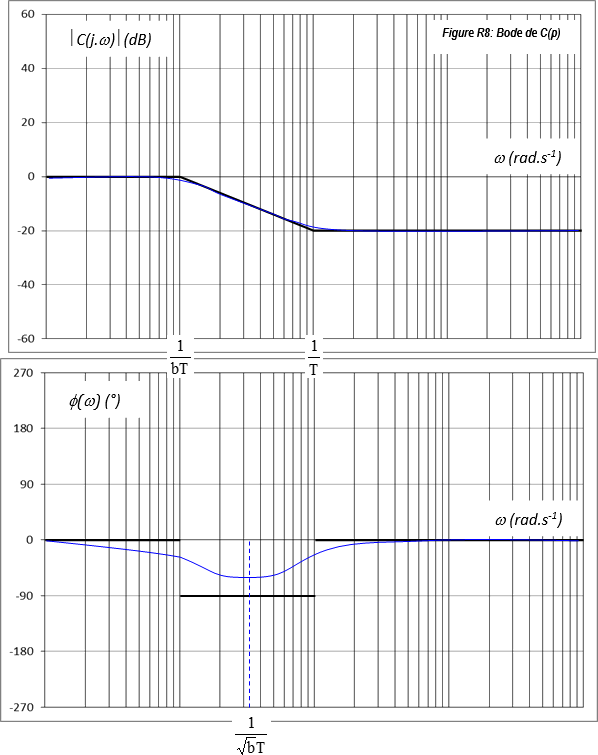
\includegraphics[width=\linewidth]{cor_05}
\end{center}
\end{minipage}

\begin{rem}
\begin{itemize}
\item En considérant que la direction du vecteur vitesse peut décrire le plan tangent au contact, la résultante des efforts $\vect{F_{12}}$ décrit alors un cône. On parle donc de cône d'adhérence. 
\item Suivant les modèles utilisés les facteurs de frottement $f_g$ lors du glissement et $f_a$ lors de l'adhérence peuvent être considérés différents. On a $f_g<f_a$.
\end{itemize}
\end{rem}

Dans le cas du Segway, dans le cas du glissement, on a, dans le cas de la roue droite, $T_{12} \vect{t_{12}} = X_D\vect{x_1}+Y_D\vect{y_1} $ soit $|T_{12}| =\sqrt{X_D^2+Y_D^2}$. On a donc 
$\sqrt{X_D^2+Y_D^2} = f Z_D$. 

Dans le cas de l'adhérence, $\sqrt{X_D^2+Y_D^2} < f Z_D$.
\end{corrige}
\else
\fi

\ifprof
\else


La stabilité du Segway impose de garantir un effort tangentiel minimal transmissible suivant $\vect{y_1}$. Par conséquent, on suppose  $Y_G = Y_F=Y_{\text{min}}$ donné. 

Le Cahier des Charges précise les valeurs minimales des rayons de courbure du virage $\rho$, définis par $|V|=\rho\dot{\phi}$, pour différentes valeurs de vitesse. Compte tenu des valeurs des paramètres géométriques et de masse du Segway, on trace sur la figure du document réponse, avec $Y_{\text{min}}=\SI{100}{N}$ et $f=0,6$, deux graphiques :
\begin{itemize}
\item  $\dfrac{\sqrt{Y_{\text{min}}+X_D^2}}{Z_D}$ en fonction de $\rho$, rayon de courbure du virage en mètre
\item  $\dfrac{Y_{\text{min}}}{Z_G}$ en fonction de $\rho$, rayon de courbure du virage en mètre.
\end{itemize}

\fi


\question{\label{q_16}En expliquant votre démarche et en complétant le document réponse, vérifier les performances attendues vis à vis des rayons de virage minimums tout en garantissant les critères de non basculement et de non dérapage.}
\ifprof
\begin{corrige}
D'une part, pour garantir le non glissement (et donc le non dérapage), il est nécessaire que $\sqrt{X_D^2+Y_D^2} < f Z_D$ soit $\dfrac{\sqrt{X_D^2+Y_D^2}}{Z_D} < f $.

D'autre part, d'aprèes la cahier des charges, on souhaite respecter l'exigence 4.3 :
\begin{itemize} 
\item circulation à  \SI{5}{km.h^{-1}} dans un virage de rayon \SI{0,5}{m};
\item circulation à  \SI{10}{km.h^{-1}} dans un virage de rayon \SI{2,5}{m};
\item circulation à  \SI{20}{km.h^{-1}} dans un virage de rayon \SI{10}{m}.
\end{itemize}
On déduit de la courbe de gauche le rayon de frottement doit être supérieur à 0,5 pour ne pas déraper (pire des cas, circulation à   \SI{20}{km.h^{-1}} dans un virage de rayon \SI{10}{m}).


\begin{center}
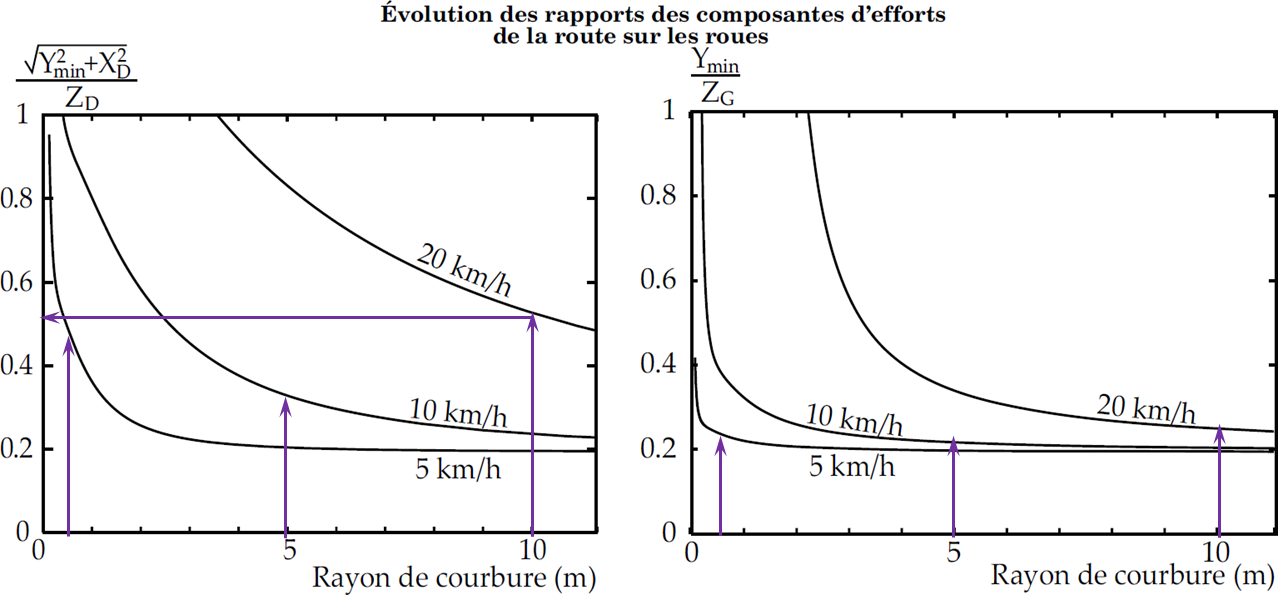
\includegraphics[width=.7\linewidth]{cor_06}
\end{center}

Vérification du non basculement ?

\end{corrige}
\else
\fi

\section{Validation de l'exigence 1 : permettre au conducteur de se déplacer aisément sur la route}

\begin{obj}
Déterminer la relation entre l’inclinaison du conducteur et l’accélération du Segway en ligne droite ainsi que les équations mécaniques nécessaires au modèle d’asservissement d’inclinaison.
\end{obj}

\ifprof
\else

Pour une utilisation confortable et sûre, le Segway doit satisfaire les performances de vitesse et d’accélération énoncées dans le \autoref{tab_02} extrait du cahier des charges.


\begin{figure}[H]
\centering
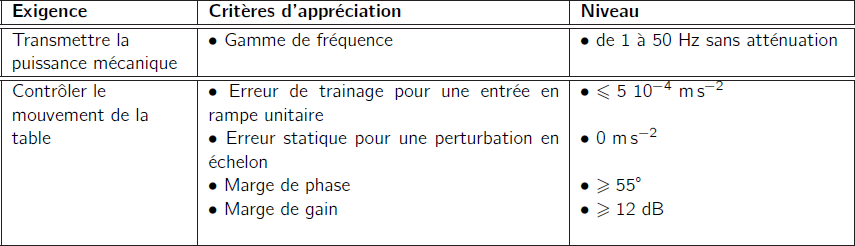
\includegraphics[width=\linewidth]{req_01}
\caption{Extrait du CdCF relatif à l'exigence 1 \label{tab_02} }%$\vect{z_3}=$}% $\beta = 0$ soit $\vect{z_3}=\vect{z_4}$ }
\end{figure}


Hypothèses :
\begin{itemize}
\item le Segway  se déplace en ligne droite : $\phi=0$ et $\beta=0$. On note donc pour simplifier $\theta_D=\theta_G = \theta$;
\item l’angle $\alpha$ d’inclinaison du conducteur est constant : $\alpha=$constant. Dans ce cas, $\vectv{A}{2}{0}=V\vect{y_1}=-R\left(\dot{\psi}+\dot{\theta}\right) \vect{y_1}$.
\end{itemize}

\fi

\subsection{Détermination des équations mécaniques régissant le système}

\ifprof
\else

On pose pour la suite les notations suivantes.

\begin{itemize}
\item Conducteur : $H$ : 
\begin{itemize}
\item centre de gravité $G$ avec $\vect{AG}=h\vect{z_4}$ et $h=\SI{0,95}{m}$ et $m_H = \SI{80}{kg}$;
\item $\inertie{G}{H} = \matinertie{A_H}{B_H}{C_H}{0}{0}{0}{\left(\vect{x_4},\vect{y_4},\vect{z_4}\right)}$ avec $A_H =\SI{18}{kg.m^2}$, $B_H =\SI{20}{kg.m^2}$ et $C_H =\SI{1,2}{kg.m^2}$.
\end{itemize}
\item Châssis : $S$ : 
\begin{itemize}
\item centre de gravité $A$ avec $m_S = \SI{25}{kg}$;
\item $A_S =\SI{0,8}{kg.m^2}$ -- moment d'inertie du châssis autour de l'axe $\left(A;\vect{x_1} \right)$; %\inertie{A}{S} = \matinertie{A_S}{B_S}{C_S}{0}{0}{0}{\left(\vect{x_1},\vect{y_2},\vect{z_2}\right)}$ avec $A_S =\SI{0,8}{kg.m^2}$, $B_Z =\SI{1,2}{kg.m^2}$ et $C_S =\SI{1,3}{kg.m^2}$.
\end{itemize}
\item Roue gauche : $R_G$ : 
\begin{itemize}
\item centre de gravité $O_G$ avec $\vect{AO_G}=\dfrac{L}{2}\vect{x_1}$, rayon $R=\SI{240}{mm}$, $L=\SI{650}{mm}$ et $m_R = \SI{5}{kg}$;
\item $A_R =\SI{0,28}{kg.m^2}$ -- moment d'inertie de la roue autour de l'axe $\left(A;\vect{x_1} \right)$; %\item $\inertie{O_G}{R_G} = \matinertie{A_R}{B_R}{C_R}{0}{0}{0}{\left(\vect{x_1},\vect{y_G},\vect{z_G}\right)}$ avec $A_R =\SI{0,28}{kg.m^2}$, $B_R =\SI{0,05}{kg.m^2}$ et $C_R =\SI{0,05}{kg.m^2}$.
\end{itemize}
\item Roue droite : $R_D$ : 
\begin{itemize}
\item centre de gravité $O_D$ avec $\vect{O_DA}=\dfrac{L}{2}\vect{x_1}$, rayon $R=\SI{240}{mm}$, $L=\SI{650}{mm}$ et $m_R = \SI{5}{kg}$;
\item $A_R =\SI{0,28}{kg.m^2}$ -- moment d'inertie de la roue autour de l'axe $\left(A;\vect{x_1} \right)$. %\item $\inertie{O_D}{R_D} = \matinertie{A_R}{B_R}{C_R}{0}{0}{0}{\left(\vect{x_1},\vect{y_D},\vect{z_D}\right)}$ avec $A_R =\SI{0,28}{kg.m^2}$, $B_R =\SI{0,05}{kg.m^2}$ et $C_R =\SI{0,05}{kg.m^2}$.
\end{itemize}
\end{itemize}


La masse et l’inertie de la motorisation et de son réducteur associé sont supposées négligeables. Le moto-réducteur fait partie du châssis.
\begin{itemize}
\item L’action mécanique exercée par la route sur les roues est modélisée par  
$\torseurstat{T}{\text{Route}}{R_G} = \torseurl{Y_G\vect{y_1}+Z_G\vect{z_0}}{\vect{0}}{I_G}$
 et  
$\torseurstat{T}{\text{Route}}{R_D} = \torseurl{Y_D\vect{y_1}+Z_D\vect{z_0}}{\vect{0}}{I_D}$.
\item L’action mécanique exercée par l'arbre de sortie du moto-réducteur sur la roue, identique pour chaque roue est modélisée par :  
$\torseurstat{T}{\text{Motoréducteur}}{R_D}
= \torseurstat{T}{\text{Motoréducteur}}{R_G}
 = \torseurl{\vect{0}}{C_S\vect{x_1}}{A}$.
 \end{itemize}
Dans cette partie, le problème est supposé plan dans $\left(A,\vect{y_1},\vect{z_0}\right)$.

\fi
\question{\label{q_17}Justifier l'hypothèse de problème plan du point de vue des efforts.}
\ifprof
\begin{corrige}
On considère que le Segway roule en ligne droite et toutes les rotations sont autour de $\vect{x_1}$; donc le mouvement est dans le plan $\left(A,\vect{y_1},\vect{z_0}\right)$.

Les actions mécaniques sont toutes dans le plan $\left(A,\vect{y_1},\vect{z_0}\right)$ (efforts dans ce même plan et moment suivant $\vect{x_1}$).


\end{corrige}
\else
\fi

\question{\label{q_18}Déterminer pour chaque solide (Conducteur, Châssis, Roue Gauche et Roue Droite) dans leur mouvement par rapport au repère Galiléen $R_0$ :}
\textit{
\begin{itemize}
\item $\vectrd{H}{0}=m_H\vectg{G}{H}{0}$;
\item $\vectrd{S}{0}=m_S\vectg{A}{S}{0}$;
\item $\vectrd{R_D}{0}=m_R\vectg{O_D}{R_D}{0}$ et $\vectrd{R_G}{0}=m_R\vectg{O_G}{R_G}{0}$;
\item $\vectrd{S}{0}\cdot \vect{y_1} = \vectrd{H}{0} \cdot\vect{y_1}+\vectrd{S}{0} \cdot\vect{y_1}+\vectrd{R_D}{0} \cdot\vect{y_1}+\vectrd{R_G}{0} \cdot\vect{y_1} $.
\end{itemize}}
\ifprof
\begin{corrige}
On a $\vectv{A}{H}{0} =\vectv{A}{2}{0} $. Par suite, $\vectv{G}{2}{0}=\vectv{A}{2}{0}+\vect{GA}\wedge \vecto{2}{0}$. 
On a donc $\vectv{G}{H}{0} = V\vect{y_1} - h \vect{z_4}\wedge \dot{\psi}\vect{x_1} $ 
$= V\vect{y_1} - h\dot{\psi} \vect{y_3}$.

En conséquence, $\vectg{G}{H}{0} = \dot{V}\vect{y_1} - h\ddot{\psi} \vect{y_3}- h\dot{\psi}^2 \vect{z_3}$ soit $\vectrd{H}{0}=m_H \left(  \dot{V}\vect{y_1} - h\ddot{\psi} \vect{y_3}- h\dot{\psi}^2 \vect{z_3}\right)$.

Enfin, $\vectrd{H}{0} \cdot\vect{y_1} = m_H \left(  \dot{V} - h\ddot{\psi} \vect{y_3}\cdot\vect{y_1}- h\dot{\psi}^2 \vect{z_3}\cdot\vect{y_1}\right)$
$= m_H \left(  \dot{V} - h\ddot{\psi}\cos\left( \alpha + \psi \right)- h\dot{\psi}^2 \sin\left( \alpha + \psi \right)\right)$.

On a  $\vectrd{S}{0}= m_S\left[\dfrac{\dd \vectv{A}{S}{0}}{\dd t}\right]_{R_0}  =m_S\dot{V} \vect{y_1}$.

De même, $\vectrd{R_D}{0}=m_R\vectg{O_G}{R_G}{0}= m_R \dot{V} \vect{y_1}$


\end{corrige}
\else
\fi


\question{\label{q_18}Déterminer pour chaque solide (Conducteur, Châssis, Roue Gauche et Roue Droite) dans leur mouvement par rapport au repère Galiléen $R_0$ :}
\textit{
\begin{itemize}  
\item $\vectmd{A}{H}{0}\cdot \vect{x_1} = \left(A_H+m_H h^2\right)\ddot{\psi} - m_H h\dot{V}\cos\left(\alpha + \psi\right)$;% -- \textbf{question pour 5/2 :)} ;
\item $\vectmd{A}{S}{0}\cdot \vect{x_1}$;
\item $\vectmd{A}{R_D}{0}\cdot \vect{x_1}$ et $\vectmd{A}{R_G}{0}\cdot \vect{x_1}$.
\end{itemize}}

\ifprof
\begin{corrige}

\textbf{Calcul de $\vectmd{A}{H}{0}\cdot \vect{x_1}$}
Méthode : 
\begin{itemize}
\item dérivation du moment cinétique en G;
\item déplacement en $A$;
\item projection sur $\vect{x_1}$.
\end{itemize}

$\vectmd{A}{H}{0}\cdot \vect{x_1} = \left(\vectmd{G}{H}{0} + \vect{AG}\wedge m_H  \vectg{G}{H}{0} \right)\cdot \vect{x_1}$
$ = \left[\dfrac{\dd \vectmc{G}{H}{0}}{\dd t}\right]_{\rep{0}} \cdot \vect{x_1}+ \left(\vect{AG}\wedge m_H  \vectg{G}{H}{0}\right) \cdot \vect{x_1} $


$ = \left[\dfrac{\dd \vectmc{G}{H}{0}\cdot \vect{x_1}}{\dd t}\right]
- \vectmc{G}{H}{0}\cdot \left[\dfrac{\dd \vect{x_1}}{\dd t}\right]_{\rep{0}}
+ \left(\vect{AG}\wedge m_H  \vectg{G}{H}{0}\right) \cdot \vect{x_1} $

$ = \left[\dfrac{\dd \dot{\psi}(t)}{\dd t}\right]
- \vect{0}
+ \left(h\vect{z_4}\wedge m_H  \left(  \dot{V}\vect{y_1} - h\ddot{\psi} \vect{y_3}- h\dot{\psi}^2 \vect{z_3}\right)\right) \cdot \vect{x_1} $

$ = A_H\ddot{\psi}(t)
+ \left(h m_H  \left(  \dot{V}\vect{z_3}\wedge \vect{y_1} - h\ddot{\psi} \vect{z_3}\wedge\vect{y_3}- h\dot{\psi}^2 \vect{z_3}\wedge \vect{z_3}\right)\right) \cdot \vect{x_1} $

$ =  A_H\ddot{\psi}(t)
+ \left(h m_H  \left(  - \dot{V}\sin\left( \alpha + \psi + \pi/2 \right)  \vect{x_1} + h\ddot{\psi} \vect{x_3} \right)\right) \cdot \vect{x_1} $

$ = A_H\ddot{\psi}(t) + h m_H  \left(  - \dot{V}\cos\left( \alpha + \psi  \right)  + h\ddot{\psi}  \right) $


\textbf{Calcul de $\vectmd{A}{S}{0}\cdot \vect{x_1}$}

$\vectmd{A}{S}{0}\cdot \vect{x_1} = A_S \ddot{\psi}(t) $

\textbf{Calcul de $\vectmd{A}{R_D}{0}\cdot \vect{x_1}$}

$\vectmd{A}{R_D}{0}\cdot \vect{x_1}  =  A_R \left( \ddot{\psi}(t) + \ddot{\theta}\right) $


\end{corrige}
\else
\fi

\question{\label{q_19}Quelle séquence d’isolements, quels bilans d'actions mécaniques et quels théorèmes permettraient d'obtenir le système de deux équations suivant (aucun calcul demandé) :}
$$
\left\{
\begin{array}{l}
\left( m_H h^2 +A_H + A_S\right)\ddot{\psi} - m_H h \dot{V} \cos\left(\alpha+\psi\right) = m_H hg \sin\left(\alpha + \psi\right) - 2C_S \\
\left( m_S +m_H + 2m_R\right)\dot{V} - m_H h \ddot{\psi} \cos\left(\alpha+\psi\right) 
+ m_H h \dot{\psi}^2 \sin\left(\alpha+\psi\right) =  - 2\dfrac{A_R}{R^2}\dot{V} - 2\dfrac{C_S}{R}  \\
\end{array}
\right.
$$
\ifprof
\begin{corrige} ~\\

\begin{figure}[H]
\centering
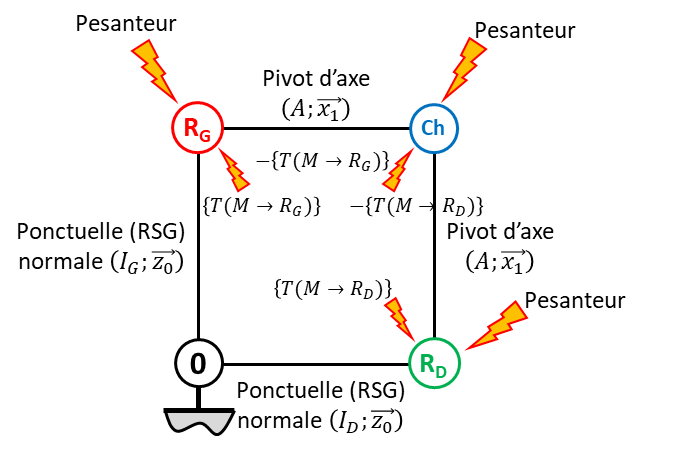
\includegraphics[width=0.5\linewidth]{cor_08}
\end{figure}

La première équation fait apparaître les couples moteur et les moments d'inertie du conducteur et du câssis. On isole donc le conducteur et le châssis. On réalise BAME.
On applique le théorème du moment dynamique en $A$ en projection sur $\vect{x_1}$.

La seconde équation fait apparaître les accélérations de chacun des solides et les moment d'inertie des roues. 
On propose d'une part d'isoler une  roue et de réaliser un théorème du moment dynamique en $A$ en projection sur $\vect{x_1}$. On obtient alors une relation entre l'action entre $Y_{DG}$ et le couple moteur.

D'autre part, on isole l'ensemble du Segway et on réalise un théorème de la résultante dynamique en projection sur l'axe  $\vect{y_1}$.

En combinant les équations (et en croisant les doigts ;)) on obtient le système d'équation donné. 

\end{corrige}
\else
\fi

%\textit{Préciser clairement pour chaque isolement le système considéré et l’équation scalaire choisie. La relation cinématique suivante, issue de la question \ref{q_08} pourra être utilisée :  $V=-R\left(\dot{\theta}+\dot{\psi}\right)$.}

\question{\label{q_20}\'Enoncer les hypothèses qui permettent d’envisager de linéariser le système précédent. Sous ces hypothèses, montrer alors que le système linéarisé peut se mettre sous la forme :}
$$
\left\{
\begin{array}{l}
A \ddot{\psi}(t) - B \dot{V}(t) = - 2C_S(t)+C\left(\alpha(t) + \psi(t)\right) \\
B \ddot{\psi}(t) - D \dot{V}(t) = 2\dfrac{C_S(t)}{R} \\\end{array}
\right.
$$
\textit{où vous préciserez les expressions des constantes $A$, $B$, $C$ et $D$. Réaliser les applications numériques.}
\ifprof
\begin{corrige}
En faisant l'hypothèse que la rotation $\alpha+\psi$ petits et en négligeant les termes d'ordre deux, on a 

$$
\left\{
\begin{array}{l}
\left( m_H h^2 +A_H + A_S\right)\ddot{\psi} - m_H h \dot{V}  = m_H hg \left(\alpha + \psi\right) - 2C_S \\
\left( m_S +m_H + 2m_R + 2\dfrac{A_R}{R^2}\right)\dot{V} - m_H h \ddot{\psi} =  - 2\dfrac{C_S}{R}  \\
\end{array}
\right. .
$$

Par identification, on a alors : $A= m_H h^2 +A_H + A_S$, $B = m_H h$, $C= m_H hg$, $D= m_S +m_H + 2m_R + 2\dfrac{A_R}{R^2}$.

AN : $A=\SI{91}{kg.m^2}$, $B=\SI{76}{kg.m}$, $C=\SI{746}{Nm}$, $D=\SI{125}{kg}$.
\end{corrige}
\else
\fi


\subsection{Relation entre l’inclinaison du conducteur et l’accélération du Segway}

On souhaite trouver la relation entre l’inclinaison $\alpha(t)$ du conducteur et l’accélération du Segway. L’asservissement est ici considéré comme parfaitement réalisé, c’est à dire $\psi=0$.

\question{\label{q_21}Montrer que cette relation s’écrit sous la forme $\dot{V}  =K\alpha(t)$ où vous préciserez la valeur numérique de $K$.}
\ifprof
\begin{corrige}
Si  $\psi=0$ on a 
$
\left\{
\begin{array}{l}
 - B \dot{V}(t) = - 2C_S(t)+C\left(\alpha(t) \right) \\
 - D \dot{V}(t) = 2\dfrac{C_S(t)}{R} \\\end{array}
\right.
$
$ \Leftrightarrow 
\left\{
\begin{array}{l}
   2C_S(t) = C\left(\alpha(t) \right) +B \dot{V}(t) \\
 - DR\dot{V}(t) = 2C_S(t) \\\end{array}
\right.
$

Soit $C\alpha(t)  +B \dot{V}(t)= - DR\dot{V}(t)$ 
$\Leftrightarrow C\alpha(t)  +\left(B + DR\right)\dot{V}(t)= 0$ 

On a donc $\alpha = - \dfrac{C}{B + DR} = -\SI{7}{m.s^{-2}.rad^{-1}}$.

\end{corrige}
\else
\fi

\question{\label{q_22}Vérifier les performances attendues du cahier des charges en vous appuyant sur les configurations proposées \autoref{fig_06}. On utilisera ici $K = -\SI{7}{m.s^{-2}.rad^{-1}}$ et on se souviendra que $V$ est négatif en marche avant.}
\ifprof
\begin{corrige}

Pour $\alpha = 22$, $\dot{V}=-7 \times 22 \times \pi /180 =\SI{2,68}{m.s^{-2}}$ ce qui est compatible avec l'accélération minimale demandée par le cahier des charges. 


Pour passer de 0 à \SI{20}{km.h^{-1}} avec l'accélération calculée, il faut $t_d = \dfrac{20 000/3600}{7}=\SI{0,8}{s}$. Sur ce laps de temps, la distance parcourue est donnée par (l'aire sous la courbe...) soit $d=0,5 t_d \times 20 000/3600 = \SI{2,2}{m}$ ce qui valide l'exigence 1.3.
\end{corrige}
\else
\fi

\ifprof
\else
\begin{figure}[H]
\centering
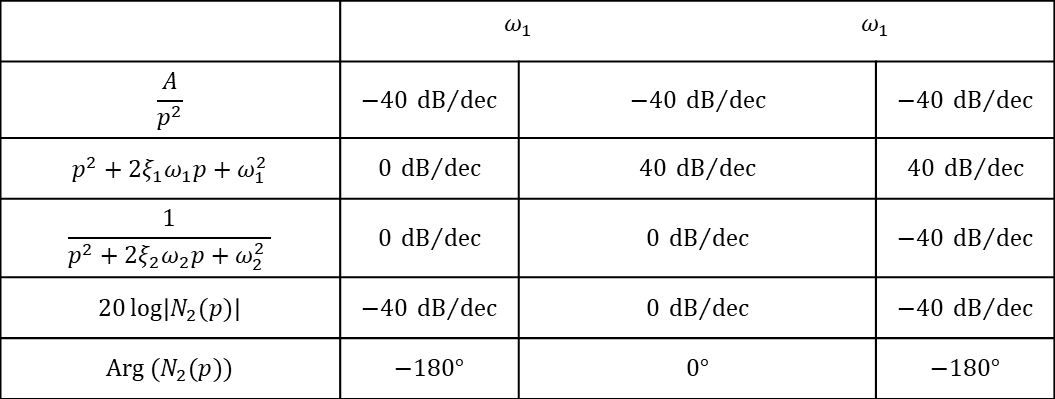
\includegraphics[width=0.9\linewidth]{fig_06}
\caption{Configurations angulaires proposées \label{fig_06}}
\end{figure}
\fi

\section{Validation de  l'exigence 2 (donner au conducteur une sensation de stabilité) et de l'exigence 3 (rester insensible aux perturbations provenant de la route)}

\begin{obj}
Vérifier les performances de l’asservissement d’inclinaison par rapport à la verticale.
\end{obj}

\ifprof
\else

Pour une utilisation confortable et sûre, le Segway doit satisfaire les performances énoncées dans la \autoref{tab_03} extrait du Cahier des Charges


\begin{figure}[H]
\centering
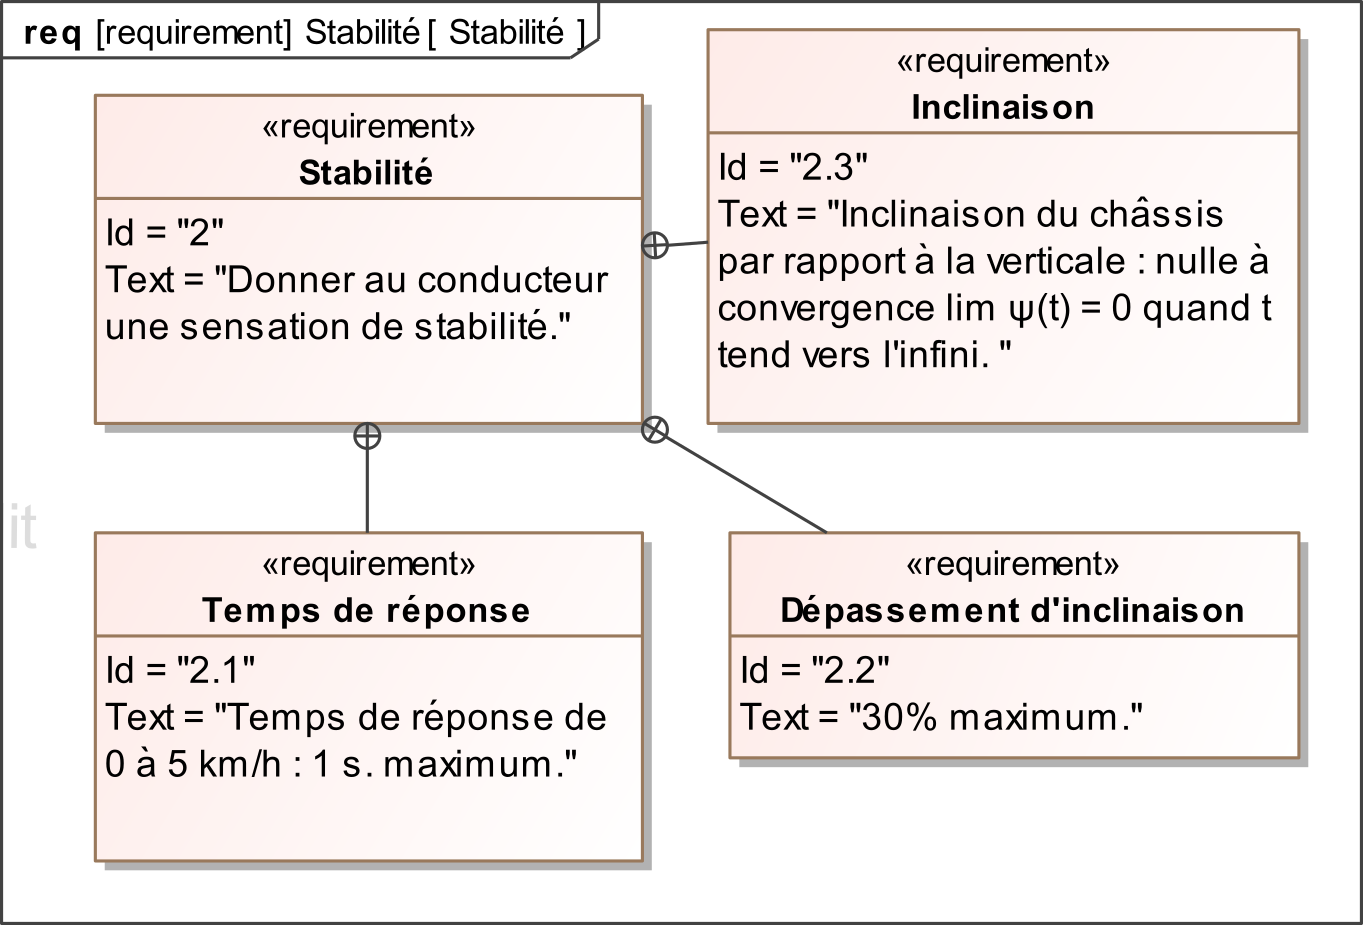
\includegraphics[height=5.5cm]{req_02}
\hfill
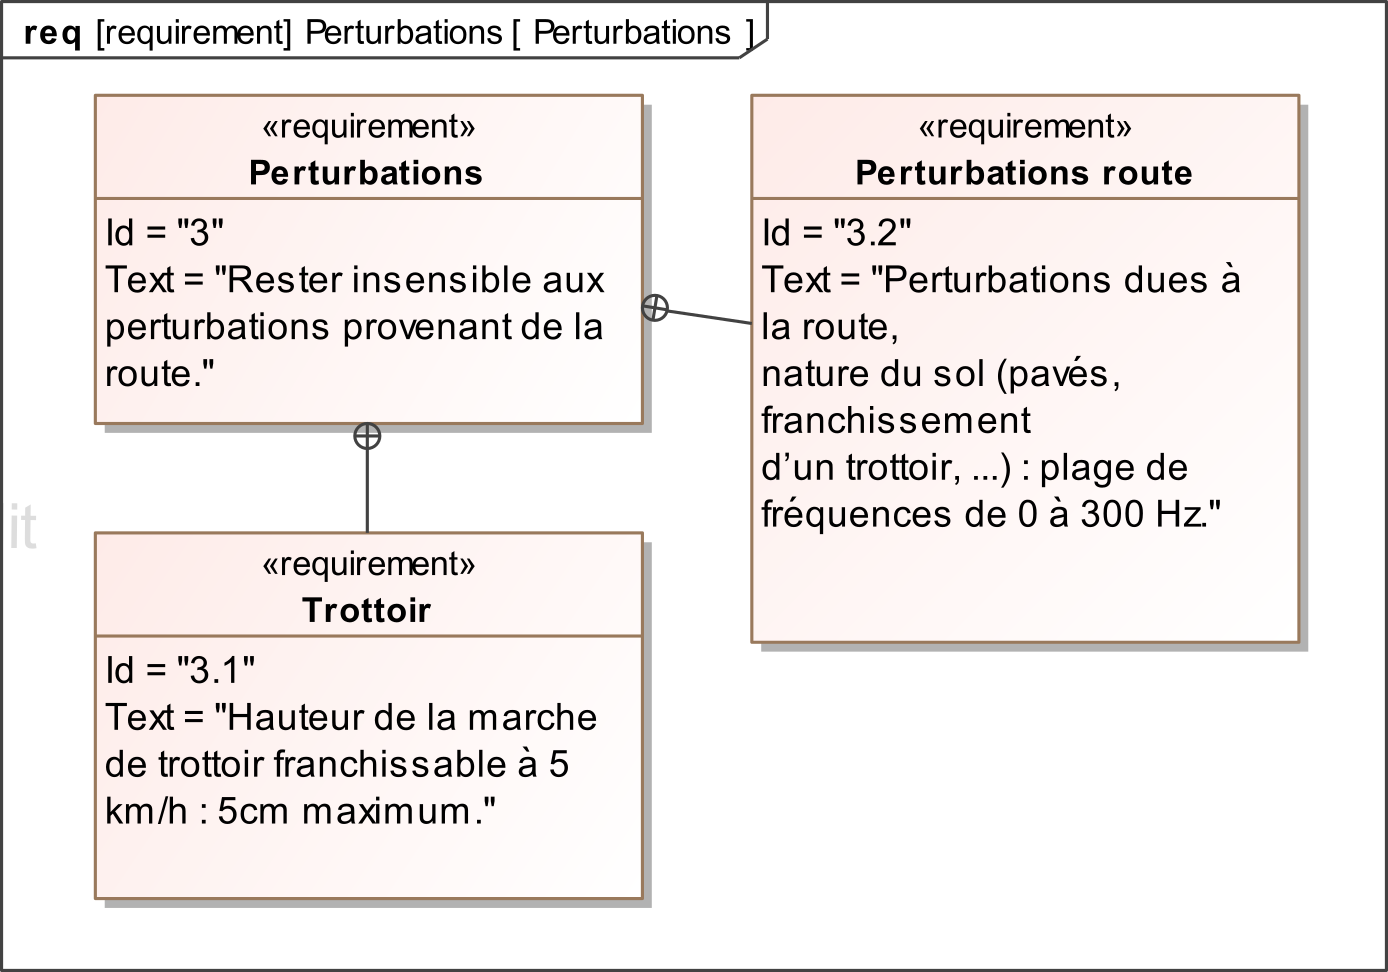
\includegraphics[height=5.5cm]{req_03}
\caption{Extrait du CdCF relatif aux exigences 2 et 3 \label{tab_03} }
\end{figure}


La régulation d’inclinaison du Segway est réalisée par :
\begin{itemize}
\item un moto-réducteur qui permet de délivrer un couple $C_m(t)=K_m u(t)$ où $u(t)$ est une grandeur de commande et  $K_m = \SI{24}{NmV^{-1}}$;
\item le système mécanique dont les équations ont été déterminées ) la question \ref{q_20} et qui peuvent, dans le cas où l’angle $\alpha(t)$ n’est pas supposé constant, se mettre sous la forme :
\end{itemize}

$
\left\{
\begin{array}{l}
\dot{V}(t) = \dfrac{1}{D} \left(B\ddot{\chi}(t)+2\dfrac{C_m(t)}{R}\right) \\
\left(DA -B^2 \right) \ddot{\chi}(t) = 2\left(\dfrac{B}{R}+D\right)C_m(t) + DC\chi(t) \\
\chi(t)=\alpha(t)+\psi(t) 
 \end{array}
\right.
$
où 
$
\left\{
\begin{array}{l}
A = \SI{90}{kg.m^2} \\
B = \SI{75}{kg.m} \\
C = \SI{750}{kg.m^2.s^{-2}} \\
D = \SI{125}{kg} \\
R = \SI{240}{mm} 
\end{array}
\right.
$.


Par commodité de signe, la notation $C_m(t)=-C_S(t)$ est utilisée dans les équations ci-dessus. Les conditions initiales sont toutes nulles.

\fi

\subsection{Stabilisation du système}
%\question{\label{q_23}Montrer que le schéma-blocs du système peut se mettre sous la forme présentée \autoref{fig_07} en déterminant l’expression littérale de $H_1(p)$.}
\question{\label{q_23}En utilisant le schéma-blocs du système présenté \autoref{fig_07} et une (ou plusieurs) des équations ci-dessus, déterminer l’expression littérale de $H_1(p)$.}

\ifprof
\begin{corrige}
D'après le schéma-blocs, $\chi(p) =C_m(p)H_1(p)$.

D'après la seconde équation, on a 
$\left(DA -B^2 \right) p^2{\chi}(p) = 2\left(\dfrac{B}{R}+D\right)C_m(p) + DC\chi(p)$
$ \Leftrightarrow \left(\left(DA -B^2 \right) p^2 -  DC \right){\chi}(p) = 2\left(\dfrac{B}{R}+D\right)C_m(p) $.

On a donc $H_1(p)=\dfrac{ 2\left(\dfrac{B}{R}+D\right)}{\left(DA -B^2 \right) p^2 -  DC}$.



\end{corrige}
\else
\fi

\ifprof
\else
\begin{figure}[H]
\centering
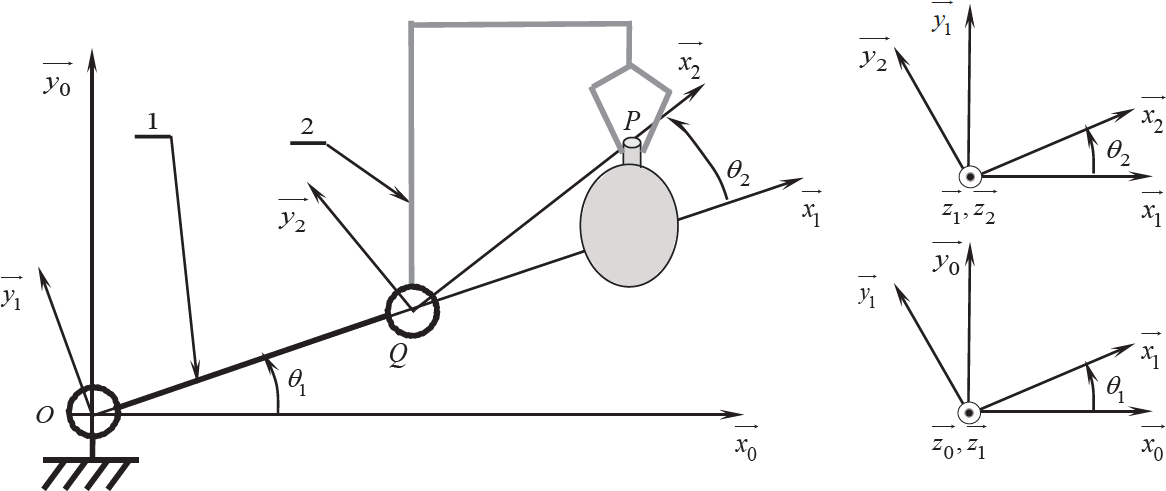
\includegraphics[width=0.6\linewidth]{fig_07}
\caption{Schéma-blocs 1 \label{fig_07}}
\end{figure}
\fi

%\question{\label{q_24}Analyser la stabilité du système d’entrée $u(t)$ et de sortie $\psi(t)$ en étudiant la fonction de transfert  $F_1(p)=\dfrac{\psi(p)}{U(p)}$. Pouvait-on s'attendre à ce résultat ?}

\question{\label{q_24}Analyser la stabilité du système d’entrée $u(t)$ et de sortie $\chi(t)$ en étudiant la fonction de transfert  $H_1(p)$. Pouvait-on s'attendre à ce résultat ?}
\ifprof
\begin{corrige}
$H_1$ a pour pôles $p_{12}=\pm\sqrt{\dfrac{DC}{DA-B^2}}$ $=\pm 4,1$. Il existe donc un pôle à partie réelle positive, le système est donc instable. 

Cette structure étant un pendule inversé (centre de gravité au dessus de l'axe des roues), on s'attendait naturellement à ce que le système soit instable.

\end{corrige}
\else
\fi


\ifprof
\else
On note alors $H_1(p)=\dfrac{K_1}{\dfrac{p^2}{\omega_1^2}-1}$. Les valeurs numériques utilisées par la suite seront : $\omega_1=\SI{4,1}{rad.s^{-1}}$  et $K_S=K_mK_1 = \SI{0,24}{rad.V^{-1}}$.

Afin de stabiliser le système, la grandeur de commande $U(p)$ est élaborée à partir des mesures de $\dot{\psi}$ (réalisée par le gyromètre), et de ${\psi}$  (réalisée par combinaison de la mesure du gyromètre et du pendule).  Le schéma-blocs obtenu est celui du document réponse (DR -- Question \ref{q_28}).
\fi


\question{\label{q_25}Dans le cas où $\alpha=0$, déterminer, en fonction de $K_S$, $k_P$, $k_V$ et $\omega_1$  la fonction de transfert $F_2(p)=\dfrac{\psi(p)}{W(p)}$. Déterminer les conditions sur $k_V$ et sur $k_P$ pour que le système soit stable.}
\ifprof
\begin{corrige}
En utilisant le schéma-blocs, on a, par fermeture de la boucle interne ($\varepsilon(p)$ : signal à la sortie du premier comparateur) :
$G_1(p)= \dfrac{\Psi(p)}{\varepsilon(p)} = \dfrac{\dfrac{K_S}{\dfrac{p^2}{\omega_1^2}-1}}{1+\dfrac{K_S}{\dfrac{p^2}{\omega_1^2}-1}pk_V}$
$\Leftrightarrow G_1(p)  = \dfrac{K_S}{{\dfrac{p^2}{\omega_1^2}-1}+K_Sk_Vp}$.

On réalise ensuite le second bouclage : $F_2(p)=\dfrac{G_1(p)}{1+G_1(p)k_P}$
$ =\dfrac{ \dfrac{K_S}{{\dfrac{p^2}{\omega_1^2}-1}+K_Sk_Vp}}{1+ \dfrac{K_S}{{\dfrac{p^2}{\omega_1^2}-1}+K_Sk_Vp}k_P} $

$ =\dfrac{K_S}{{\dfrac{p^2}{\omega_1^2}-1+K_Sk_Vp}    + K_Sk_P} $
$ =\dfrac{K_S}{{\dfrac{p^2}{\omega_1^2}+K_Sk_Vp}    + K_Sk_P-1} $

$F_2$ est d'ordre 2. pour que $F_2$ soit stable il faut nécessairement que les coefficients de $p$ soient strictement positifs. 

$K_S>0$; donc nécessairement $k_v>0$. Il faut aussi que $K_Sk_P-1>0$ donc $k_P >\dfrac{1}{K_S}$.

\end{corrige}
\else
\fi


\ifprof
\else
$F_2(p)$ est une fonction de transfert du second ordre pouvant se mettre sous la forme 
$F_2(p)=\dfrac{\psi(p)}{W(p)}=\dfrac{K_2}{1+\dfrac{2\xi}{\omega_0}p+\dfrac{p^2}{\omega_0^2}}$.
\fi


\question{\label{q_26}Déterminer, en fonction de $K_S$, $k_P$, $k_V$ et $\omega_1$ les expressions de $K_2$ et $\xi$ $\omega_0$.}
\ifprof
\begin{corrige}
En mettant $F_2(p)$ sous forme canonique, on a donc
$ F_2=\dfrac{\dfrac{K_S}{ K_Sk_P-1}}{\dfrac{p^2}{\omega_1^2}\dfrac{1}{ K_Sk_P-1}+\dfrac{K_Sk_V}{ K_Sk_P-1}p    +1} $.
On a donc $K_2 = \dfrac{K_S}{ K_Sk_P-1}$, $\dfrac{2\xi}{\omega_0} = \dfrac{K_Sk_V}{ K_Sk_P-1}$ et $\dfrac{1}{\omega_0^2} = \dfrac{1}{\omega_1^2\left( K_Sk_P-1\right)}$.

En conséquences, $\omega_0 = \omega_1\sqrt{K_Sk_P-1}$, 
$\xi = \dfrac{K_Sk_V \omega_0}{2 \left(K_Sk_P-1\right)}$
$=\dfrac{K_Sk_V \omega_1\sqrt{K_Sk_P-1}}{2 \left(K_Sk_P-1\right)}$
$=\dfrac{K_Sk_V \omega_1}{2\sqrt{K_Sk_P-1}}$
\end{corrige}
\else
\fi

On choisit une pulsation propre $\omega_0$  proche de celle du système mécanique, c’est à dire  
$\omega_0=1,5 \omega_1 = \SI{6,15}{rad.s^{-1}}$.

\question{\label{q_27}Déterminer les valeurs de $k_V$ et de $k_P$ telles que le temps de réponse à 5\% soit minimal.}
\ifprof
\begin{corrige}
On a $\omega_0=1,5 \omega_1 =  \omega_1\sqrt{K_Sk_P-1}$ soit $1,5  = \sqrt{K_Sk_P-1}$ et $ k_P = \dfrac{1,5^2 +1}{K_S}$.

AN : $ k_P = \dfrac{1,5^2 +1}{0,24} = \SI{13,54}{V.rad^{-1}}$

Pour que le temps de réponse à 5 \% soit minimal il est nécessaire que $\xi=0,69$ soit $\xi=\dfrac{K_Sk_V \omega_1}{2\sqrt{K_Sk_P-1}}$

$\Leftrightarrow k_V = \dfrac{2\xi \sqrt{K_Sk_P-1}}{K_S \omega_1}  $

AN : $ k_V = \dfrac{2\times  0,69 \sqrt{0,24 \times 13,54-1}}{0,24 \omega_1} \simeq  \SI{2,1}{Vs}$

\end{corrige}
\else
\fi

\subsection{Asservissement d’inclinaison du chariot}

\ifprof
\else
La consigne de la régulation de l’inclinaison $\psi(t)$ du châssis par rapport à la verticale est notée $\psi_c(t)$. On introduit un correcteur de fonction de transfert $C(p)$ qui élabore le signal $w(t)$ (de transformée de Laplace $W(p)$) à partir de l’écart $\varepsilon(t)=\psi_c(t)-\psi(t)$.
\fi

\question{\label{q_28}Compléter le schéma-blocs de l’asservissement fourni sur le document réponse en faisant apparaître la régulation de l’inclinaison.}
\ifprof
\begin{corrige}~\\

\begin{figure}[H]
\centering
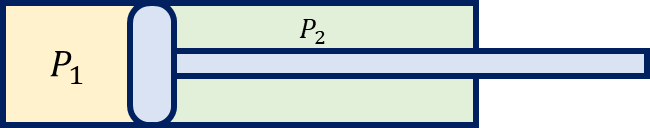
\includegraphics[width=0.7\linewidth]{cor_09}
%\caption{Réponse temporelle de $\chi(t)$ \label{fig_08}}
\end{figure}


\end{corrige}
\else
\fi

\ifprof
\else
La régulation d’inclinaison du Segway consiste à maintenir la consigne $\psi_c(t)$ nulle. Cette régulation est réalisée, si quelle que soit l’inclinaison $\alpha(t)$ du conducteur, la sortie $\psi(t)$ converge vers $\psi_c(t)$, valeur nulle ici.
Le conducteur agit directement sur la valeur de $\alpha(t)$ pour accélérer ou décélérer. Pour le système Segway, conducteur exclu, le paramètre $\alpha(t)$ peut être considérée comme une perturbation.
Un correcteur proportionnel $C(p)=K_c$ est envisagé.

\fi


\question{\label{q_30_a}Montrer que le schéma-blocs peut se mettre sous la forme suivante en explicitant $F_2(p)$ et $F_3(p)$.}
\ifprof
\else
\begin{figure}[H]
\centering
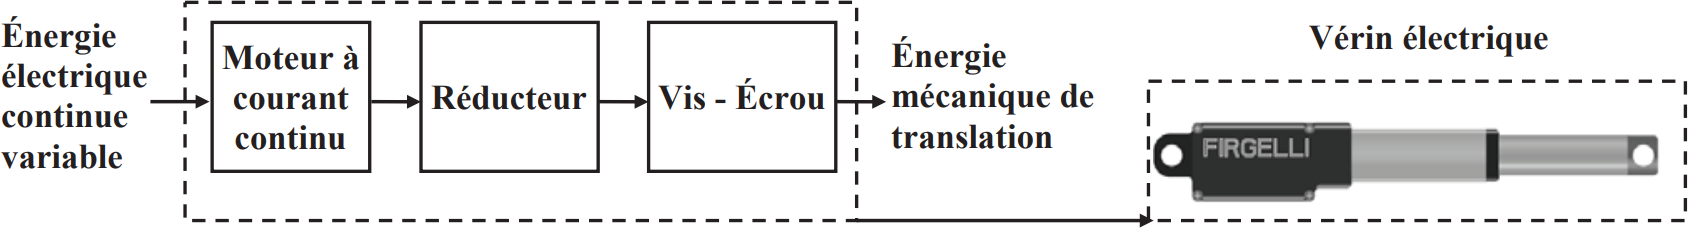
\includegraphics[width=0.6\linewidth]{fig_09}
%\caption{Réponse temporelle de $\chi(t)$ \label{fig_08}}
\end{figure}
\fi

\ifprof
\begin{corrige}~\\
Le schéma-blocs précédent est équivalent à la forme suivante. 
\begin{figure}[H]
\centering
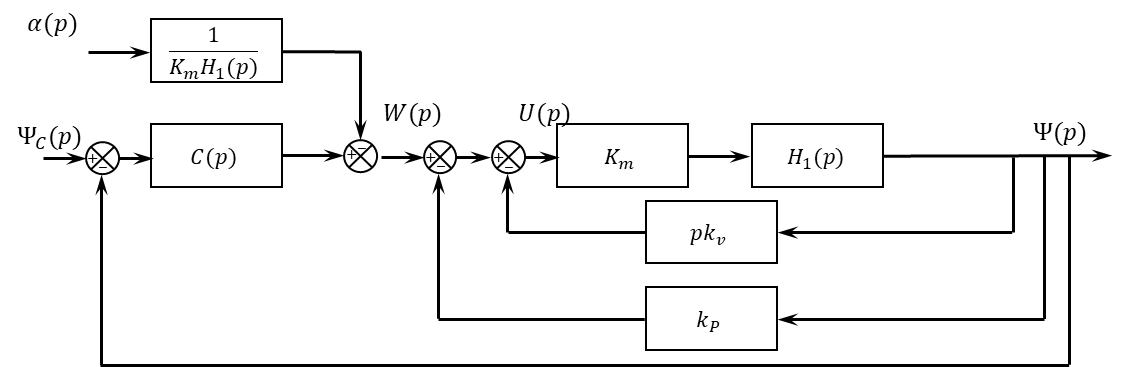
\includegraphics[width=0.7\linewidth]{cor_10}
%\caption{Réponse temporelle de $\chi(t)$ \label{fig_08}}
\end{figure}

On a donc $F_3(p)=\dfrac{1}{K_mH_1(p)}$ $=\dfrac{1}{K_m\dfrac{K_1}{\dfrac{p^2}{\omega_1^2}-1}}$
 $=\dfrac{1}{K_m\dfrac{K_1}{\dfrac{p^2-\omega_1^2}{\omega_1^2}}}$
  $=\dfrac{1}{K_m\omega_1^2\dfrac{K_1}{p^2-\omega_1^2}}$.
    $=\dfrac{p^2-\omega_1^2}{K_m\omega_1^2K_1}$.

On a alors : $\dfrac{K_m H_1(p)}{1+K_m H_1(p)pk_v}$ et donc 
$F_2(p)=\dfrac{\dfrac{K_m H_1(p)}{1+K_m H_1(p)pk_v}}{1+\dfrac{K_m H_1(p)k_P}{1+K_m H_1(p)pk_v}}$
$= \dfrac{K_m H_1(p)}{1+K_m H_1(p)pk_v+K_m H_1(p)k_P}$.


De plus $H_1(p)=\dfrac{K_1}{\dfrac{p^2}{\omega_1^2}-1}$ et donc 
$F_2(p)= \dfrac{K_m \dfrac{K_1}{\dfrac{p^2}{\omega_1^2}-1}}{1+K_m \dfrac{K_1}{\dfrac{p^2}{\omega_1^2}-1}pk_v+K_m \dfrac{K_1}{\dfrac{p^2}{\omega_1^2}-1}k_P}$

$= \dfrac{K_m K_1}{\dfrac{p^2}{\omega_1^2}-1+K_m K_1pk_v+K_m K_1k_P}$

\end{corrige}
\else
\fi

\question{\label{q_30}Calculer l’inclinaison $\psi(t)$ du châssis en régime permanent, lorsque la perturbation $\alpha(t)$ est un échelon d’amplitude $\alpha_0$. Le cahier des charges est-il satisfait ?}
\ifprof
\begin{corrige}
Lorsque $\Psi_C$ est nul, on a $\Psi (p)=F_2(p)\left( -\alpha(p) F_3(p)-\Psi(p) C(p) \right)$
soit $\Psi (p)\left(1+C(p)F_2(p)\right)=-F_2(p)  F_3(p) \alpha(p) $. On a donc
$\Psi (p)=-\dfrac{F_2(p)  F_3(p)}{1+C(p)F_2(p)} \alpha(p) $.

On a donc, $\lim\limits_{t \to +\infty} \psi (t) =\lim\limits_{p \to +0} p \Psi (p)$
$=\lim\limits_{p \to 0}  -p\dfrac{F_2(p)  F_3(p)}{1+C(p)F_2(p)} \alpha(p)$
$=\lim\limits_{p \to 0} -p\dfrac{F_2(p)  F_3(p)}{1+C(p)F_2(p)} \dfrac{\alpha_0}{p}$

$=\lim\limits_{p \to 0} -\alpha_0\dfrac{F_2(p)  F_3(p)}{1+C(p)F_2(p)} $

Or $\lim\limits_{p \to 0} F_2(p) =\dfrac{K_m K_1}{-1+K_m K_1k_P}$ et 
$\lim\limits_{p \to 0} F_3(p) =\dfrac{1}{K_mK_1}$.

On a  alors, 
$\lim\limits_{t \to +\infty} \psi (t) = -\alpha_0\dfrac{\dfrac{K_m K_1}{-1+K_m K_1k_P}\dfrac{1}{K_mK_1}}{1+\dfrac{K_m K_1}{-1+K_m K_1k_P} K_c}$
$= -\alpha_0\dfrac{1}{-1+K_m K_1k_P+K_m K_1 K_c}$.

La valeur finale de $\psi(t)$ ne tend pas vers 0. Le cahier des charges n'est pas respecté.


\end{corrige}
\else
\fi

Un correcteur proportionnel intégral $C(p)=K_i \left(1+\dfrac{1}{T_i p}\right)$ est envisagé.

\question{\label{q_31}Démontrer que ce correcteur permet de satisfaire le cahier des charges  vis-à-vis de l’écart en régime permanent pour une perturbation en échelon.}
\ifprof
\begin{corrige}
$C(p)=K_i \left(1+\dfrac{1}{T_i p}\right) = K_i \dfrac{T_i p+1}{T_i p}$

Dans ces conditions, on a 
$\lim\limits_{p \to 0} -\alpha_0\dfrac{F_2(p)  F_3(p)}{1+C(p)F_2(p)} $
$ = \lim\limits_{p \to 0} -\alpha_0\dfrac{F_2(p)  F_3(p)}{1+K_i \dfrac{T_i p+1}{T_i p}F_2(p)} $
$ = \lim\limits_{p \to 0} -\alpha_0\dfrac{T_i p F_2(p)  F_3(p)}{T_i p+K_i \left(T_i p+1\right)F_2(p)} $
$ = \lim\limits_{p \to 0} -\alpha_0\dfrac{T_i p \dfrac{K_m K_1}{-1+K_m K_1k_P}  \dfrac{1}{K_mK_1}}{T_i p+K_i \left(T_i p+1\right)\dfrac{K_m K_1}{-1+K_m K_1k_P}}  = 0$.
\end{corrige}
\else
\fi

On souhaite dimensionner le correcteur. Pour cela, on étudie le schéma-blocs construit en question \ref{q_28} et on considère alors $\alpha(t)=0$. La Fonction de Transfert en Boucle Ouverte est pour cet asservissement : $\text{FTBO}(p)=C(p)F_2(p)$.

\question{\label{q_29}Justifier l'allure du diagramme de Bode de $F_2(p)$ donné sur le document réponse.}
\ifprof
\begin{corrige}
On a $F_2(p)= \dfrac{K_m K_1}{\dfrac{p^2}{\omega_1^2}-1+K_m K_1pk_v+K_m K_1k_P}$
$ = \dfrac{\dfrac{K_m K_1}{K_m K_1k_P-1}}{\dfrac{p^2}{\left(K_m K_1k_P-1\right)\omega_1^2}+\dfrac{K_m K_1k_v}{K_m K_1k_P-1}p+1}$.

$F_2(p)$ est un système d'ordre 2. 
Le gain tend vers $20\log \left(\dfrac{K_m K_1}{K_m K_1k_P-1}\right)$. Si $\xi<1$, la pente est alors 
de $-\SI{40}{dB/decade}$ à partir de la pulsation $\omega_0 = \omega_1\sqrt{K_m K_1k_P-1}$.

AN : $\omega_0 = 4,1\sqrt{0,24 \times 13,54-1} \simeq \SI{6,13}{rad/s}$.


\end{corrige}
\else
\fi


\question{\label{q_29_a}En analysant le diagramme de Bode de $F_2(p)$ que peut-on dire de la stabilité (et des marges de stabilité) du système ?}
\ifprof
\begin{corrige}
Le gain étant toujours inférieur à \SI{0}{dB} et la phase étant toujours supérieure à 180\degres. Le système est stable.
\end{corrige}
\else
\fi


\question{\label{q_29_bis}Tracer les diagrammes de Bode asymptotiques de la fonction de transfert du correcteur $C(p)$, en utilisant les paramètres $K_i$ et $T_i$. Préciser les valeurs caractéristiques sur les diagrammes.}
\ifprof
\begin{corrige}
 $C(p)=\dfrac{K_i}{T_i} \dfrac{1+T_i p}{ p} $.  
 Pour le tracer, prenons $T_i=\SI{1}{s}$ et $K_i = 1$. Pour $\omega=\SI{10e-2}{rad.s^{-1}}$, on a alors  $F_2(p) \simeq \dfrac{K_i}{T_i p}$. On a alors : 
 $G_{\text{dB}}(F_2) = -20 \log 10^{-2} = \SI{40}{dB} $.
 

 Lorsque $\omega$ tend vers l'infini, le gain tend vers $20\log K_i$.


\begin{figure}[H]
\centering
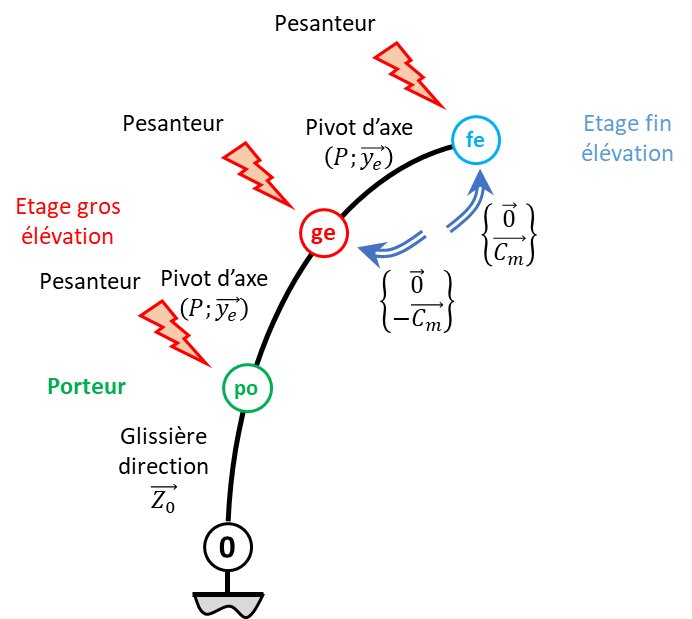
\includegraphics[width=0.7\linewidth]{cor_11}
%\caption{Réponse temporelle de $\chi(t)$ \label{fig_08}}
\end{figure}


\begin{figure}[H]
\centering
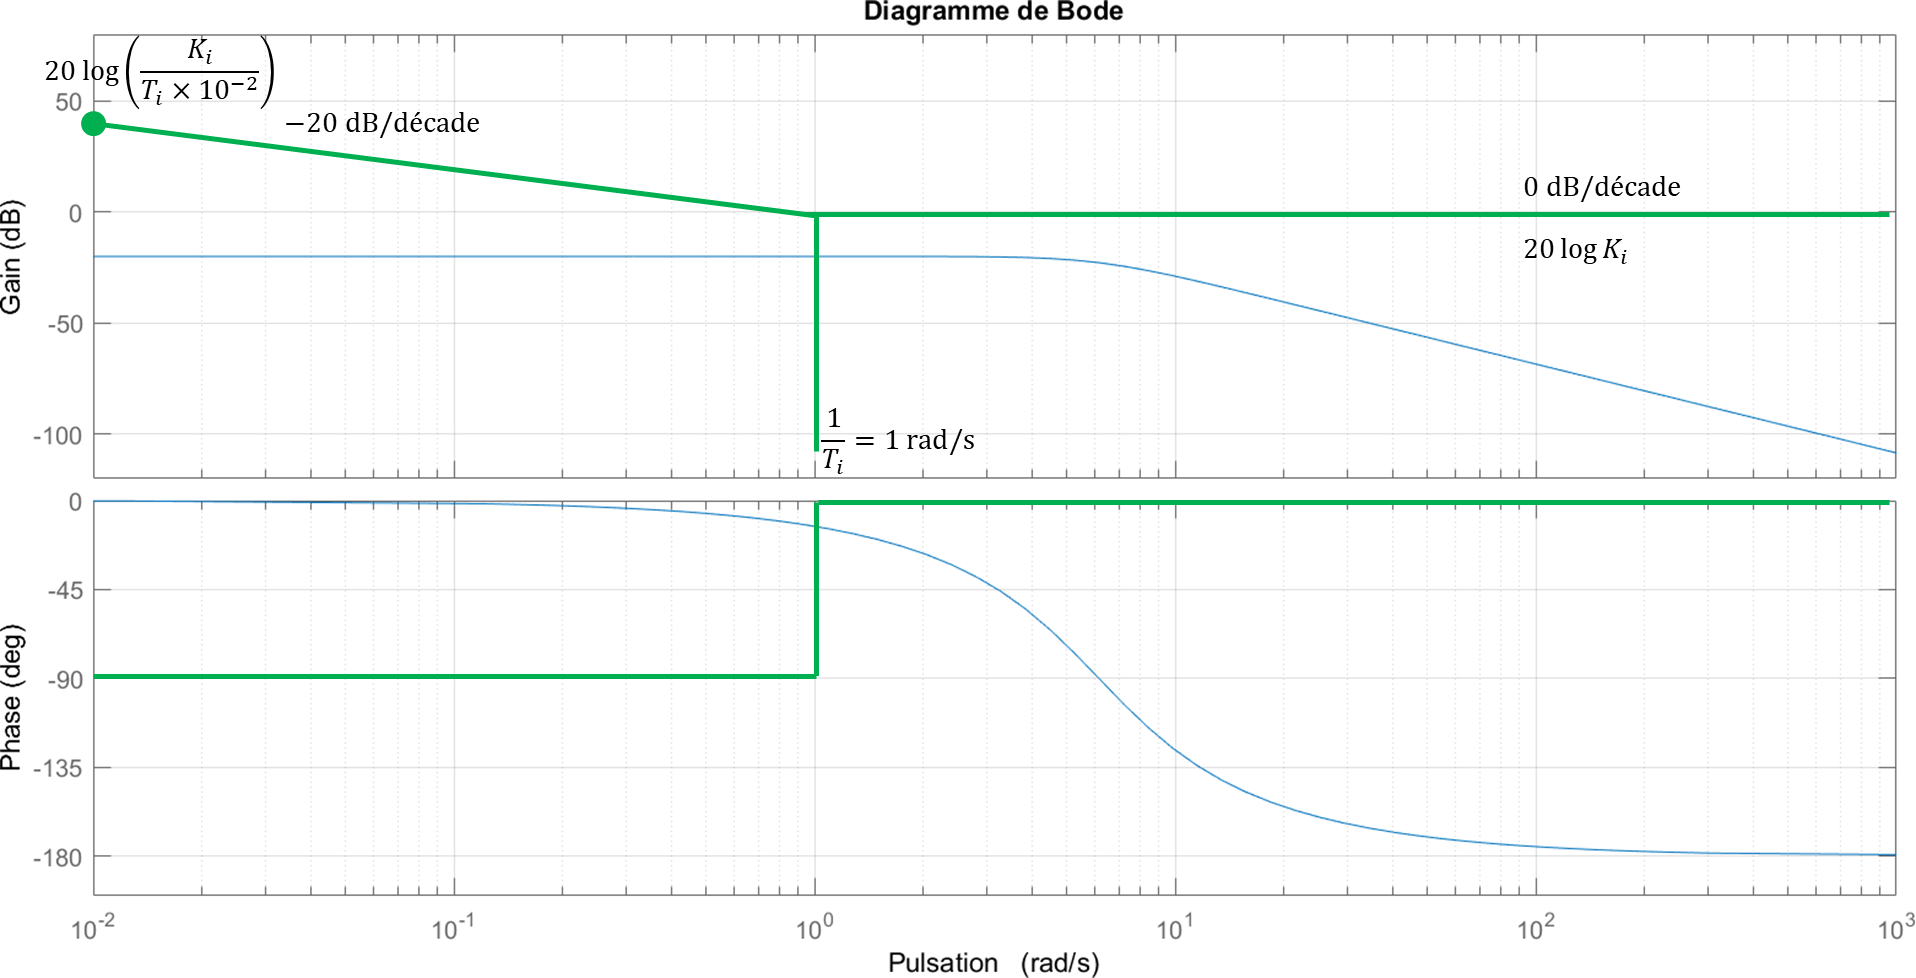
\includegraphics[width=0.7\linewidth]{cor_12}
%\caption{Réponse temporelle de $\chi(t)$ \label{fig_08}}
\end{figure}
 
\end{corrige}
\else
\fi

On impose $\omega_i = \dfrac{1}{T_i}=\dfrac{\omega_c}{10}$ où $\omega_c$ est la pulsation de coupure à \SI{0}{dB} de la FTBO corrigée par le correcteur proportionnel intégral.

\question{\label{q_32}Déterminer graphiquement $\omega_c$ telle que la marge de la $\text{FTBO}(p)$ soit $M_{\phi}=45\degres$. En déduire la valeur de $T_i$.}
\ifprof
\begin{corrige}~\\
\begin{enumerate}
\item On repère la marge de phase de 45\degres.
\item On recherche la pulsation pour laquelle la phase vaut -135\degres : $\omega_c = \SI{12}{rad.s^{-1}}$.
\item On détermine le gain actuel pour cette pulsation : il vaut $-\SI{25}{dB}$ (non demandé ici). 
\end{enumerate}

On a  $\omega_c = \SI{12}{rad.s^{-1}}$; donc $T_i = 10/\omega_c = \SI{0,83}{s}$.

\begin{figure}[H]
\centering
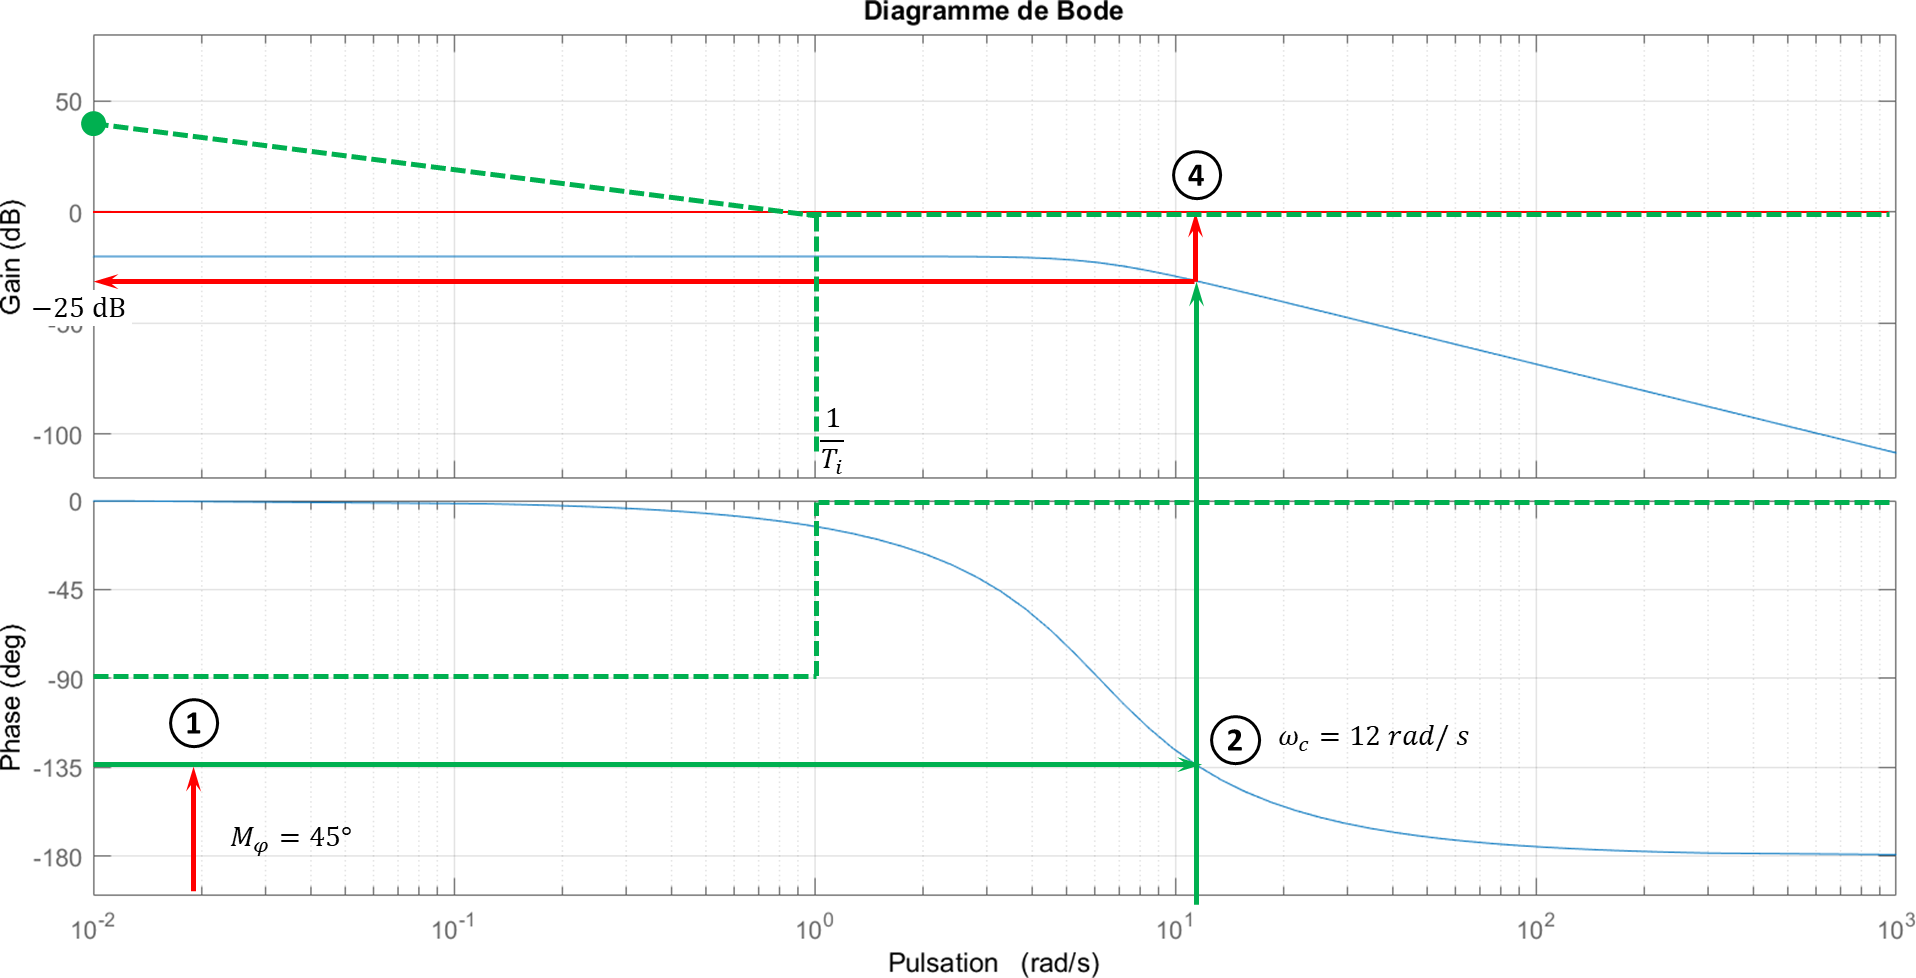
\includegraphics[width=0.7\linewidth]{cor_13}
%\caption{Réponse temporelle de $\chi(t)$ \label{fig_08}}
\end{figure}



\end{corrige}
\else
\fi

\question{\label{q_32_bis}Déterminer analytiquement $\omega_c$ telle que la marge de la $\text{FTBO}(p)$ soit $M_{\phi}=45\degres$. En déduire la valeur de $T_i$.}
\ifprof
\begin{corrige}
On cherche $\omega_c$ tel que $\varphi(\omega_c)=-135\degres$ avec $\varphi(\omega)=\text{Arg}\left(\text{FTBO}(p)\right)$ $ =\text{Arg}\left(C(p)\cdot {F_2}(p)\right)$. 

... Calcul...


\end{corrige}
\else
\fi

\question{\label{q_33}Déterminer alors $K_i$ tel que $\omega_c$ soit effectivement la pulsation de coupure à \SI{0}{dB} de la FTBO corrigée.}
\ifprof
\begin{corrige} ~\\

\textbf{Graphiquement}

Le gain du correcteur tend vers $20 \log K_i $. On cherche $K_i$ tel que $20 \log K_i = 25$; donc $K_i = 10^{\dfrac{25}{20}}  = 17,78$.


\textbf{Analytiquement}
(...)
\end{corrige}
\else
\fi

\subsection{Vérification graphique des performances attendues}
\ifprof
\else
Le modèle de comportement précédent est utilisé en simulation pour vérifier le pré-dimensionnement. Les performances de la correction sont étudiées grâce aux évolutions de $\chi(t)=\alpha(t)+\psi(t)$, qui représente l’angle d’inclinaison du conducteur par rapport à la verticale. La consigne $\alpha(t)$, imposée par le conducteur, est un échelon d’amplitude 20\degres. Après réglages définitifs, l’évolution temporelle est obtenue \autoref{fig_08}. 
\fi

\ifprof
\else
\begin{figure}[H]
\centering
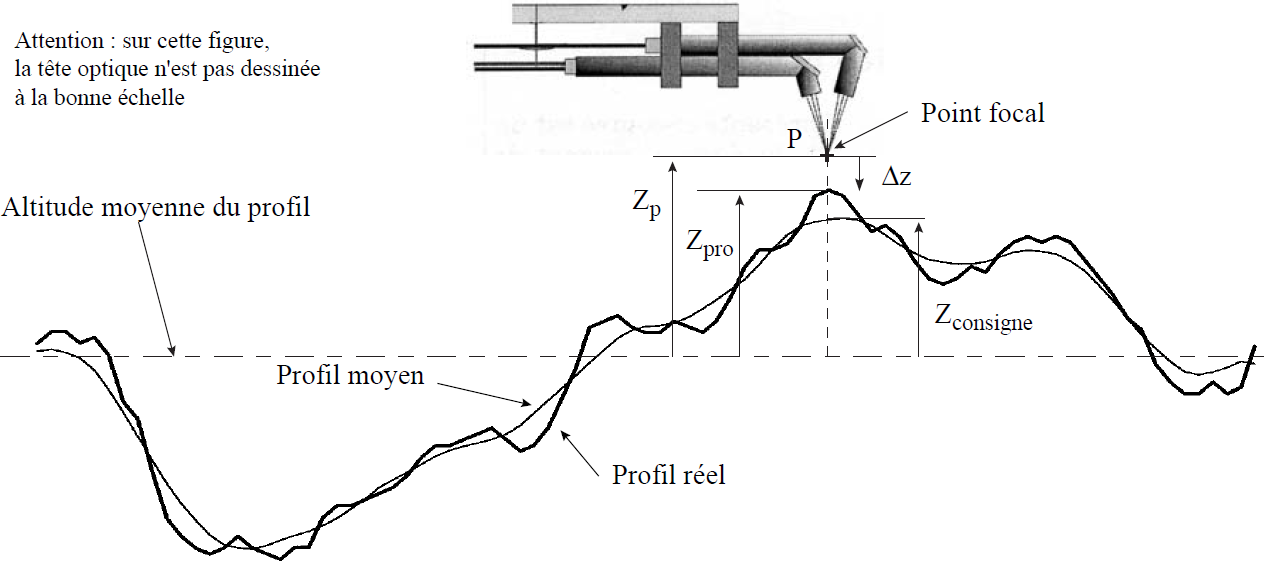
\includegraphics[width=0.6\linewidth]{fig_08}
\caption{Réponse temporelle de $\chi(t)$ \label{fig_08}}
\end{figure}
\fi

%%%%%%%%%%%%%%%%%%%%%%%%%%%%%%%%%%%%%%
\question{\label{q_34}Conclure quant au respect des critères de dépassement et de précision associés à l'exigence 2.}
\ifprof
\begin{corrige}

On a vu que correcteur PI permettait que l'exigence 2.3 soit satisfaite. La réponse temporelle ci-dessous permet d'affirmer que les exigences 2.1 et 2.2 sont satisfaites également.


\begin{figure}[H]
\centering
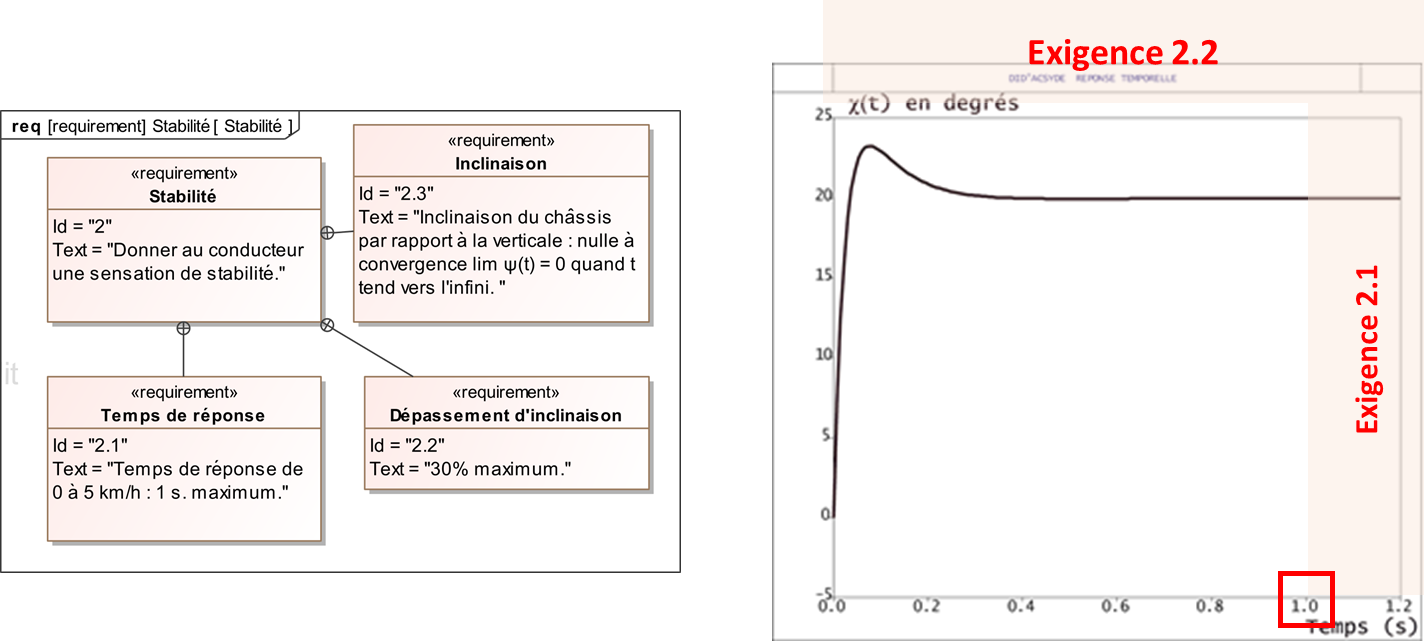
\includegraphics[width=0.7\linewidth]{cor_14}
%\caption{Réponse temporelle de $\chi(t)$ \label{fig_08}}
\end{figure}

\end{corrige}
\else
\fi


\ifprof
\else

\newpage 
\section*{Document de réponse}

\textbf{Question \ref{q_04}}

\begin{figure}[H]
\centering
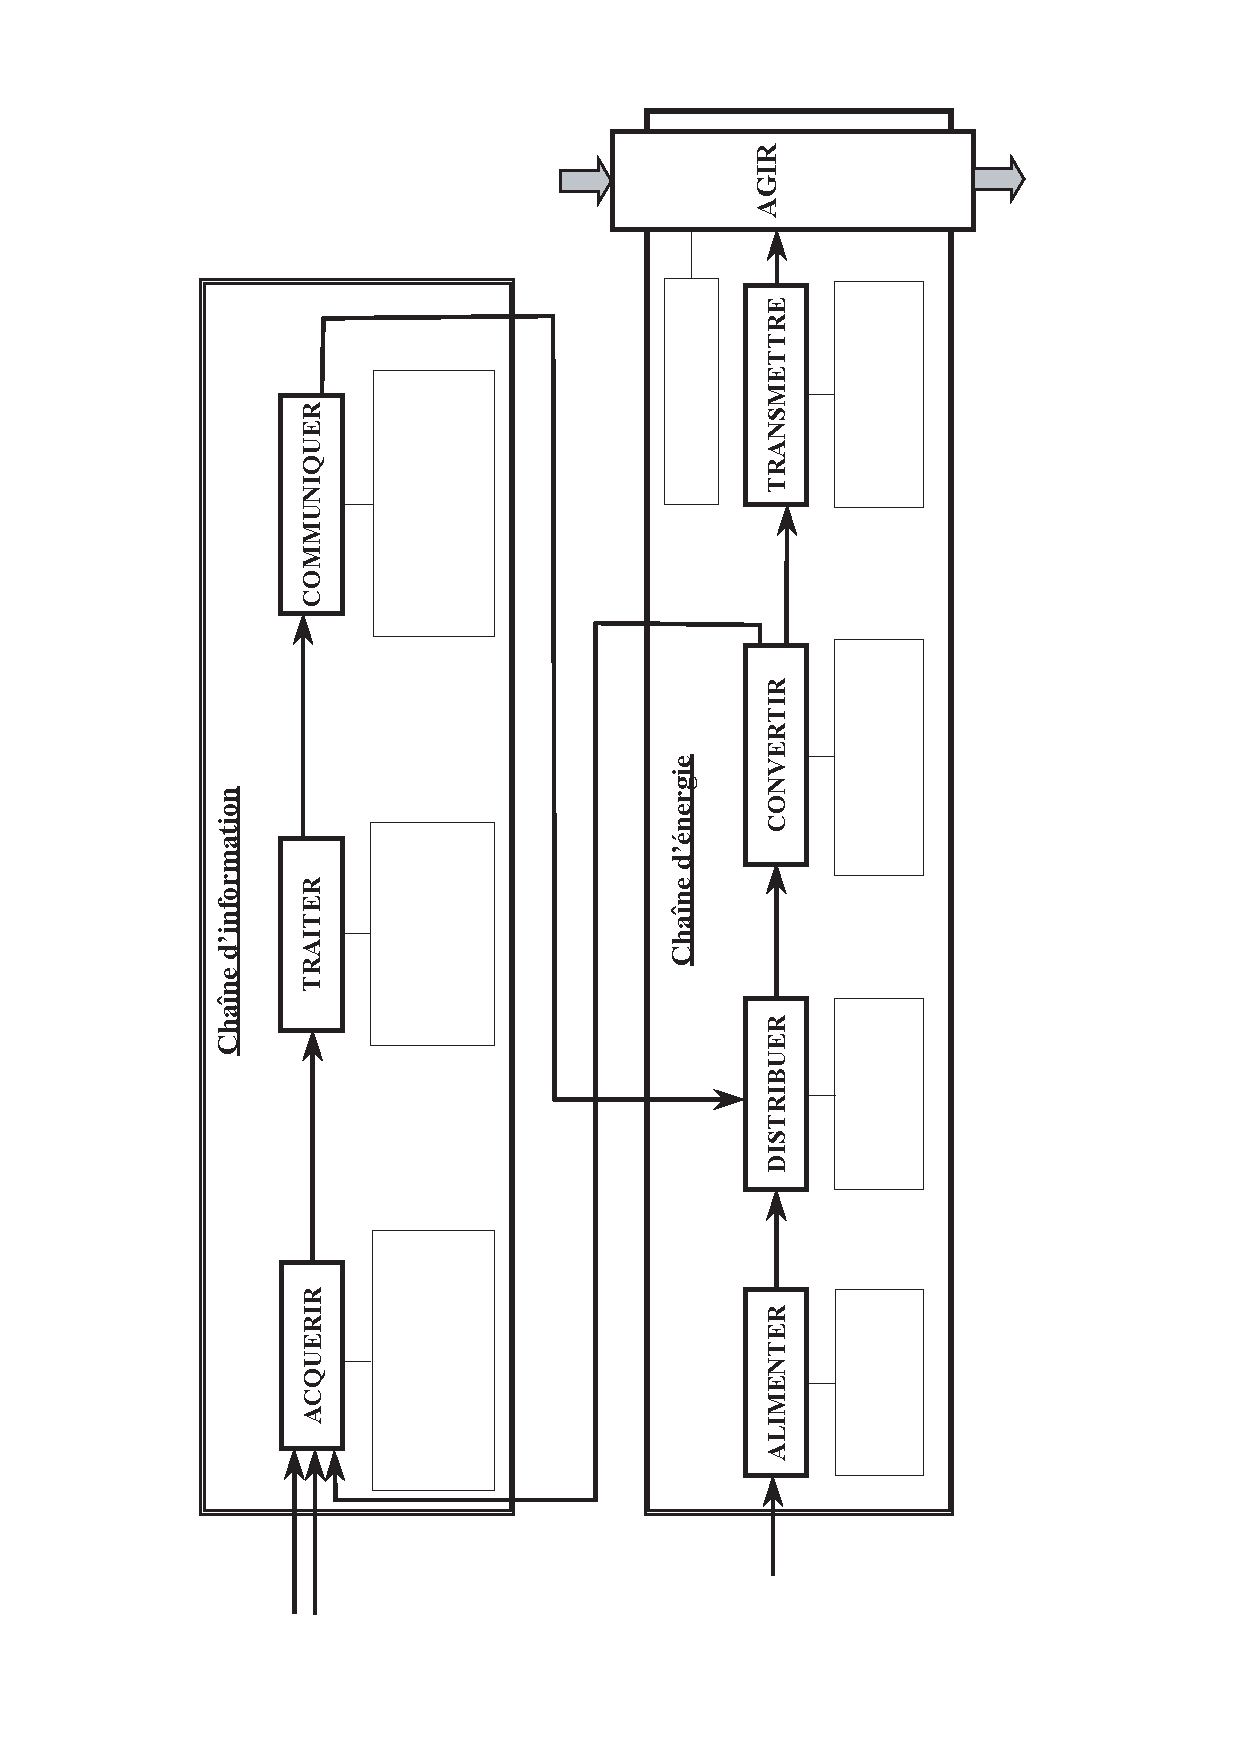
\includegraphics[width=.8\linewidth]{dr_01.pdf}
\end{figure}

\textbf{Question \ref{q_06}}
\begin{figure}[H]
\centering
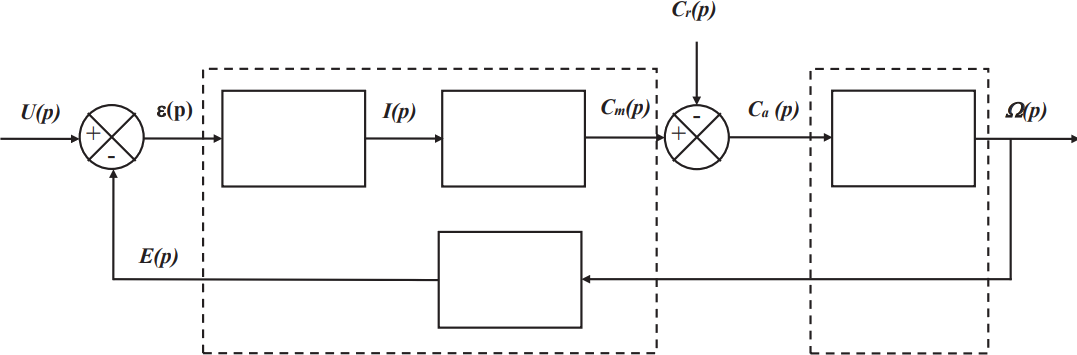
\includegraphics[width=.7\linewidth]{dr_01.png}
\end{figure}


\newpage


\textbf{Question \ref{q_10}}
\begin{figure}[H]
\centering
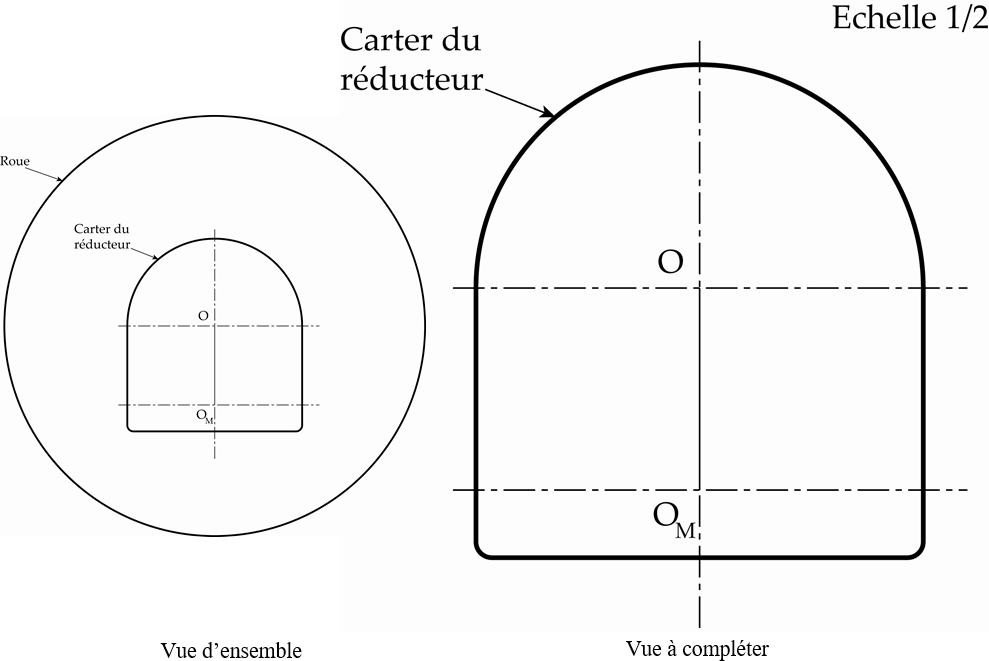
\includegraphics[width=.9\linewidth]{dr_02}
\end{figure}


\textbf{Question \ref{q_12}}

\begin{figure}[H]
\centering
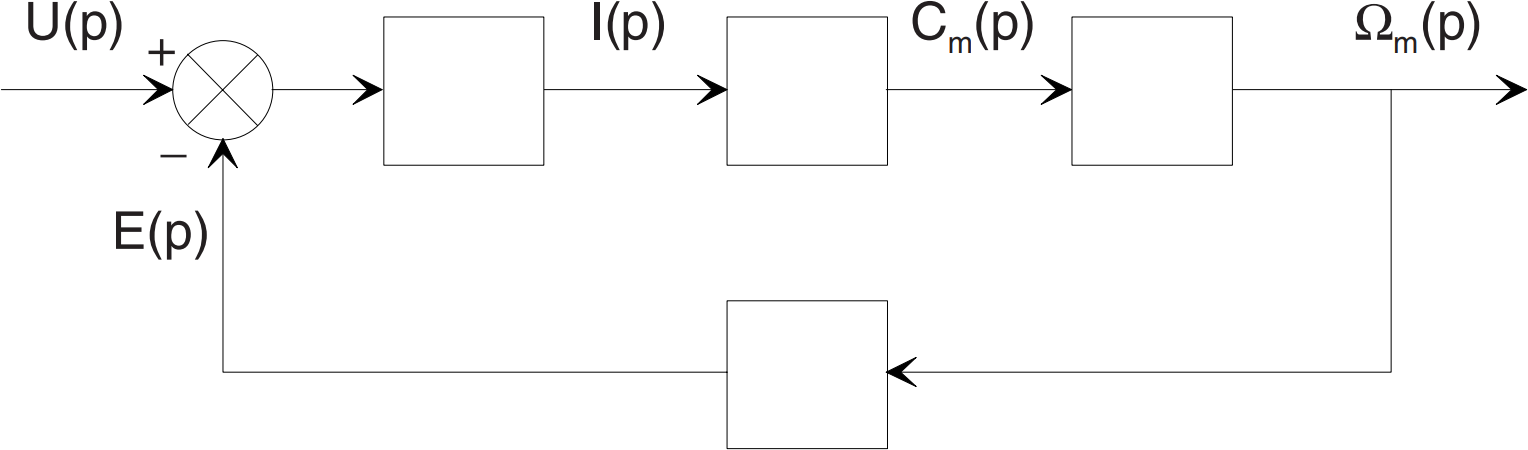
\includegraphics[width=.8\linewidth]{dr_03}
\end{figure}


\textbf{Question \ref{q_16}}

\begin{figure}[H]
\centering
{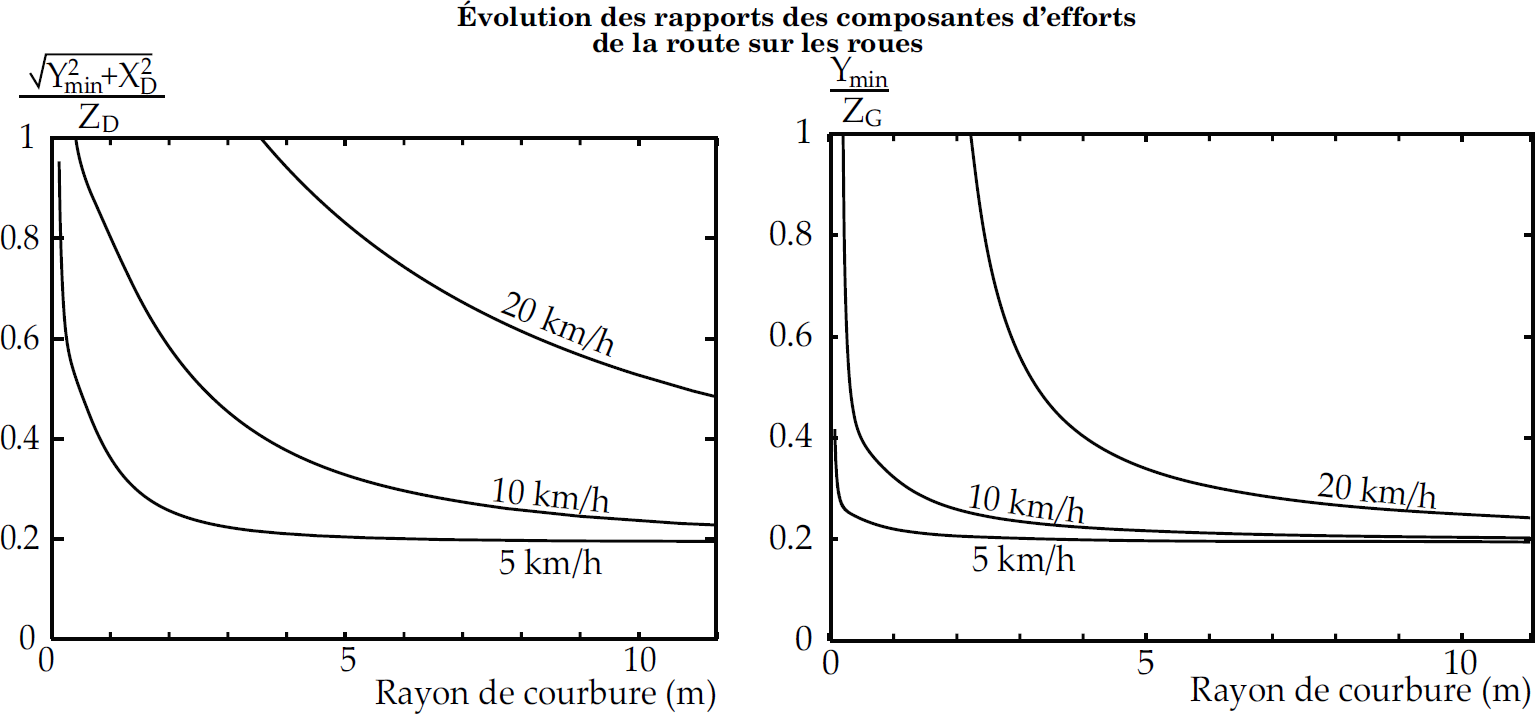
\includegraphics[width=.8\linewidth]{dr_06.png}}
\end{figure}


\newpage

\textbf{Question \ref{q_28}}

\begin{figure}[H]
\centering
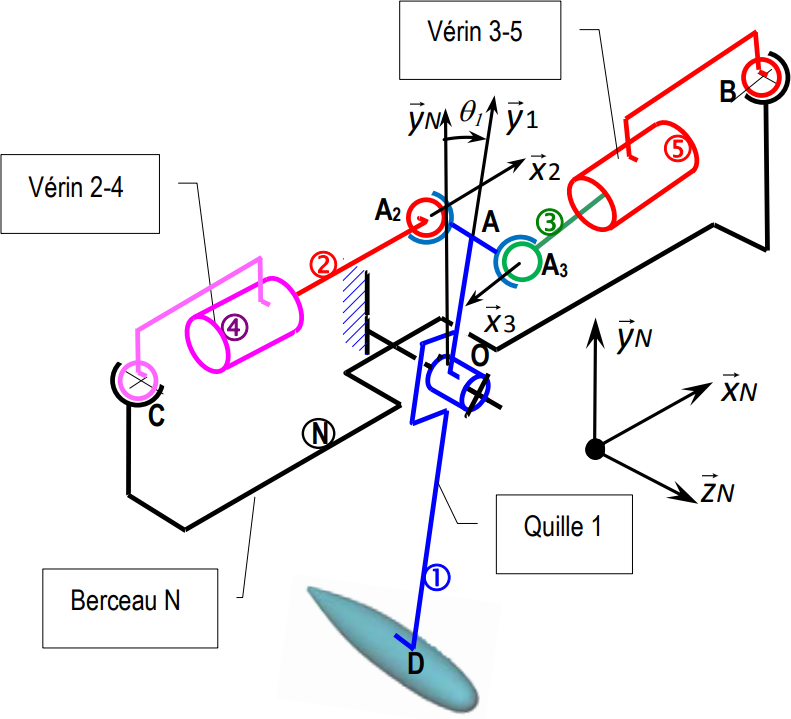
\includegraphics[width=.7\linewidth]{dr_05}
\end{figure}

\vspace{3cm}




\textbf{Question \ref{q_29}}

\begin{figure}[H]
\centering
{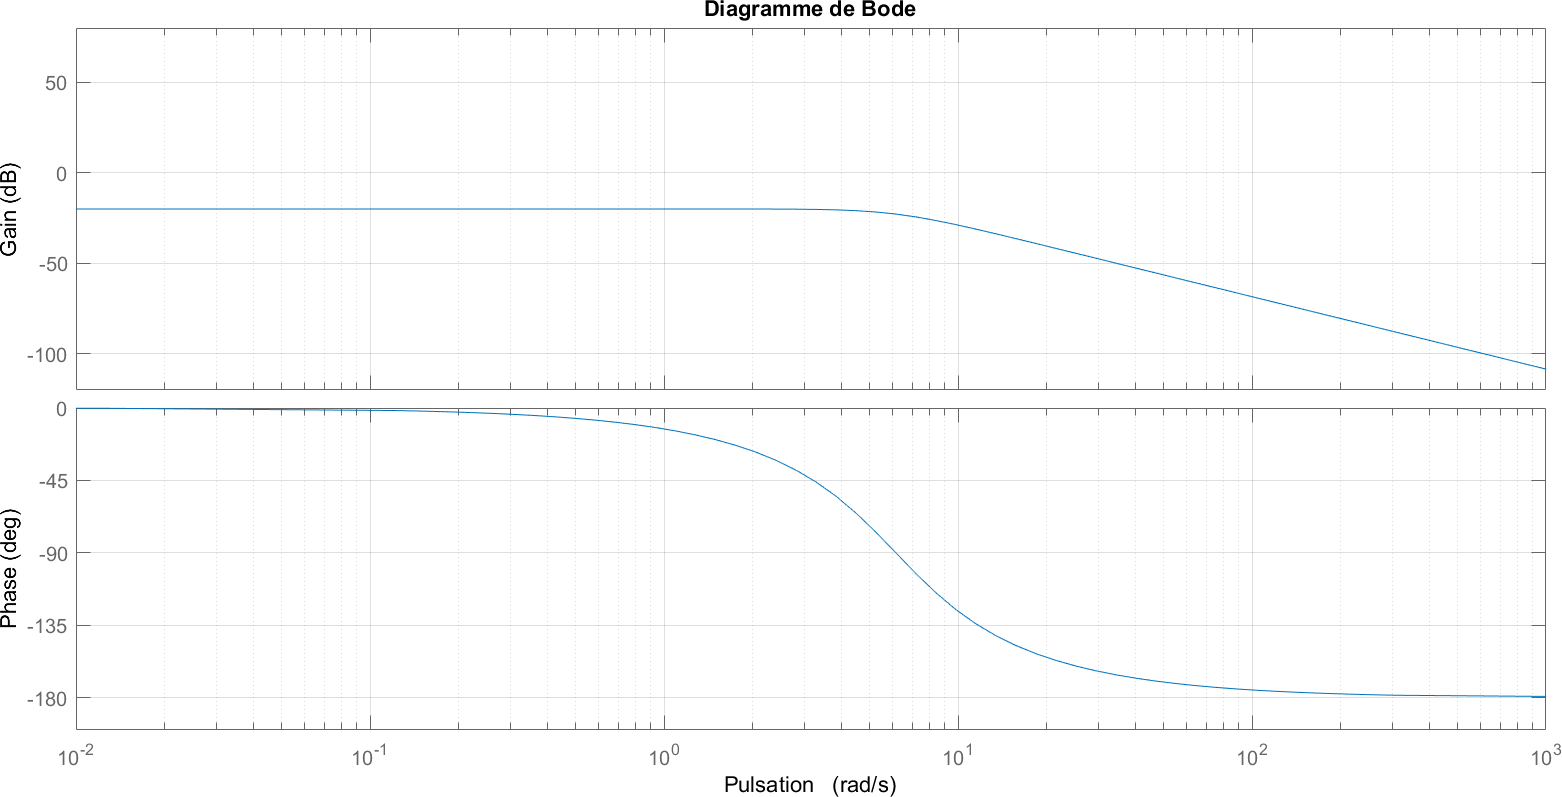
\includegraphics[width=.9\linewidth]{Bode.png}}
\end{figure}

\fi
